\documentclass[11pt,a4paper]{article}
\usepackage[margin=20mm,headheight=22pt]{geometry}
\usepackage[T1]{fontenc}
\usepackage[utf8]{inputenc}
\usepackage{lmodern}
\usepackage{microtype}
\usepackage{graphicx}
\usepackage{pdflscape}
\usepackage{booktabs}
\usepackage{longtable}
\usepackage{tabularx}
\usepackage{array}
\usepackage{amsmath,amssymb}
\usepackage{xcolor}
\usepackage{caption}
\usepackage{float}
\usepackage{enumitem}
\usepackage{fancyhdr}
\usepackage{titlesec}
\usepackage{hyperref}
\usepackage{url}
\usepackage{listings}

\definecolor{TInk}{HTML}{261F2B}
\definecolor{TMuted}{HTML}{665E6B}
\definecolor{TBrand}{HTML}{8B2463}
\definecolor{TBrandSoft}{HTML}{F5E7F0}
\definecolor{TCritical}{HTML}{B63A2B}
\definecolor{TSafe}{HTML}{287B5B}
\definecolor{TInfo}{HTML}{276DA7}
\definecolor{TLine}{HTML}{DDD7E0}
\definecolor{TPaper}{HTML}{FBF9FB}

\hypersetup{colorlinks=true,linkcolor=TBrand,citecolor=TInfo,urlcolor=TInfo,pdftitle={TriageLoop: A Safety-Oriented, Deadline-Aware Control Loop for Emergency-Department Waiting Rooms},pdfauthor={TriageLoop Team}}
\urlstyle{same}
\setlength{\parindent}{0pt}
\setlength{\parskip}{5.5pt}
\setlength{\tabcolsep}{5pt}
\renewcommand{\arraystretch}{1.18}
\setlist[itemize]{leftmargin=16pt,itemsep=2pt,topsep=3pt}
\setlist[enumerate]{leftmargin=18pt,itemsep=2pt,topsep=3pt}
\captionsetup{font=small,labelfont={bf,color=TBrand}}
\titleformat{\section}{\Large\bfseries\color{TInk}}{\thesection}{0.55em}{}
\titleformat{\subsection}{\large\bfseries\color{TInk}}{\thesubsection}{0.55em}{}
\titleformat{\subsubsection}{\normalsize\bfseries\color{TBrand}}{\thesubsubsection}{0.55em}{}
\pagestyle{fancy}
\fancyhf{}
\lhead{\small\textcolor{TMuted}{TriageLoop Technical Monograph}}
\rhead{\small\textcolor{TMuted}{Accenture Innovation Challenge 2026}}
\cfoot{\small\textcolor{TMuted}{\thepage}}
\renewcommand{\headrulewidth}{0.3pt}
\renewcommand{\headrule}{\hbox to\headwidth{\color{TLine}\leaders\hrule height \headrulewidth\hfill}}

\newcommand{\prototype}{\textbf{Synthetic decision-support prototype - not validated for clinical use.}}
\newcommand{\code}[1]{\nolinkurl{#1}}
\newcommand{\finding}[1]{\colorbox{TBrandSoft}{\parbox{0.95\linewidth}{#1}}}
\newcolumntype{Y}{>{\raggedright\arraybackslash}X}
\newcolumntype{L}[1]{>{\raggedright\arraybackslash}p{#1}}
\newcolumntype{C}[1]{>{\centering\arraybackslash}p{#1}}
\lstset{basicstyle=\ttfamily\small,breaklines=true,frame=single,rulecolor=\color{TLine},backgroundcolor=\color{TPaper},columns=fullflexible,showstringspaces=false}

\begin{document}

\begin{titlepage}
\pagecolor{TPaper}
\color{TInk}
\vspace*{18mm}
{\Large\bfseries\color{TBrand} TRIAGELOOP.AI\par}
\vspace{7mm}
{\LARGE\bfseries A Safety-Oriented, Deadline-Aware Control Loop\par}
\vspace{2mm}
{\LARGE\bfseries for Emergency-Department Waiting Rooms\par}
\vspace{5mm}
{\Large Technical Working Paper and Reproducibility Monograph\par}
\vspace{12mm}
\noindent\colorbox{TBrand}{\parbox{0.94\textwidth}{\vspace{4mm}\color{white}\Large\bfseries Patient need becomes time. Time is tested against capacity. A clinician closes the loop.\vspace{4mm}}}
\vfill
\begin{tabular}{@{}ll@{}}
Prepared for: & Accenture Innovation Challenge 2026 - Round 2 \\
Problem track: & PatientTriage.ai \\
System version: & Prototype 0.4.0 / Model 2.0.0 / Simulation 1.1.0 \\
Evidence lock: & 22 August 2026 \\
Document status: & Technical release candidate \\
Authors: & TriageLoop Team \\
\end{tabular}
\vspace{10mm}

\prototype

\textit{This document reports engineering and synthetic-simulation evidence. It does not establish clinical effectiveness, patient benefit, safe staffing, legal compliance, or production readiness.}
\end{titlepage}
\nopagecolor

\begin{abstract}
Emergency-department triage is usually represented as a one-time severity classification made at arrival. The real waiting-room safety problem is temporal: a patient's condition and the department's ability to respond can both change after that classification. TriageLoop is a nurse-led research prototype that converts repeated observations into a conservative patient-specific \emph{Dynamic Action Window}, estimates whether the live queue can meet that window, and exposes the difference as \emph{Clinical Slack}. Its quantitative path combines age-aware deterministic rules, calibrated discrete-time trajectory risk, class-conditional conformal prediction, out-of-distribution checks, a discrete-event Queue Twin, and a bounded Next Best Observation mechanism. A clinician may accept, modify, or override every recommendation; material events are stored in a recomputed SHA-256 hash chain.

The work was developed under a predeclared evaluation protocol using 10,000 seeded synthetic longitudinal encounters, 30,020 time-indexed snapshots, 28 curated edge cases, three site profiles, and paired queue simulations. The selected compact boosted-hazard model passed the registered synthetic recall, calibration, and critical-class coverage gates. Across 1,200 policy shifts under simulated 3x load, TriageLoop reduced Action Window misses by 20.5\% (95\% CI 17.4\%-23.8\%) versus fixed 15-minute periodic re-triage. The effect remained directionally positive at 10-, 20-, and 30-minute response definitions, although only the 30-minute definition exceeded 20\%. The single-observation hypothesis failed: it requested 87.5\% fewer observations but lost 7.1 percentage points of operational critical recall. The product consequently releases Next Best Observation only as a first step, with full reassessment or escalation as the required fallback. An open MIMIC-IV demo supplied a bounded input-scale plausibility check over 63,163 measurements; it is not ED or clinical validation.

Two independent Claude review cycles were handled as red-team inputs rather than authority. Verified findings produced a stronger comparator, explicit alert-workload reporting, corrected explanation attribution, response-window sensitivity, six additional product surfaces, and a retained Docker clean-machine release gate. The final prototype passed 73 automated tests, TypeScript verification, an optimized production build, and a browser-verified deterioration-to-audit journey. The contribution is not a claim to have invented AI triage or dynamic queues; it is a safety-oriented recomposition that keeps clinical need, uncertainty, operational feasibility, human authority, and evidentiary limitations visible in one control loop.
\end{abstract}

\vspace{3mm}
\textbf{Keywords:} emergency-department triage; clinical deterioration; conformal prediction; discrete-time hazard; queue simulation; deadline scheduling; human-in-the-loop; uncertainty; safety engineering; synthetic evaluation.

\clearpage
\tableofcontents
\listoffigures
\listoftables
\vspace{4mm}
\noindent\colorbox{TBrandSoft}{\parbox{0.96\textwidth}{
\textbf{Visual technical map.} The three principal blueprints are deliberately presented on dedicated pages: the complete layered system architecture (Figure~\ref{fig:architecture}), the online runtime decision pipeline (Figure~\ref{fig:runtimepipeline}), and the offline ML development/validation pipeline (Figure~\ref{fig:mlpipeline}).
}}
\clearpage

\section{Executive Technical Synopsis}

TriageLoop is built around a distinction that is easy to miss: clinical urgency and operational feasibility are related, but they are not the same variable. A patient's need determines when an action should occur. Capacity determines whether the department is likely to meet that requirement. Queue optimization must never make the clinical requirement appear less urgent.

The system therefore answers six questions in sequence:

\begin{enumerate}
  \item What has changed in this waiting patient?
  \item Do deterministic age-aware safety rules require immediate action?
  \item What is the calibrated trajectory of near-term escalation risk, and how uncertain is it?
  \item By when should the next specified clinical action occur?
  \item Given current resources and queue state, will that time requirement be met?
  \item What does the clinician decide, and what evidence must be preserved?
\end{enumerate}

The corresponding operating quantities are:

\begin{align}
W_i(t) &= \min\{W_{\mathrm{rule}}, W_{\mathrm{category}}, W_{\mathrm{model}}, W_{\mathrm{safe\ mode}}\}, \\
S_i(t) &= W_i(t) - \widehat{\eta}_i(t),
\end{align}

where $W_i(t)$ is the maximum recommended delay to the next action for patient $i$, $\widehat{\eta}_i(t)$ is the Queue Twin's projected time to that action, and $S_i(t)$ is Clinical Slack. Negative Slack is not a diagnosis; it is a visible capacity conflict.

\clearpage
\begin{landscape}
\thispagestyle{fancy}
\vspace*{\fill}
\begin{center}
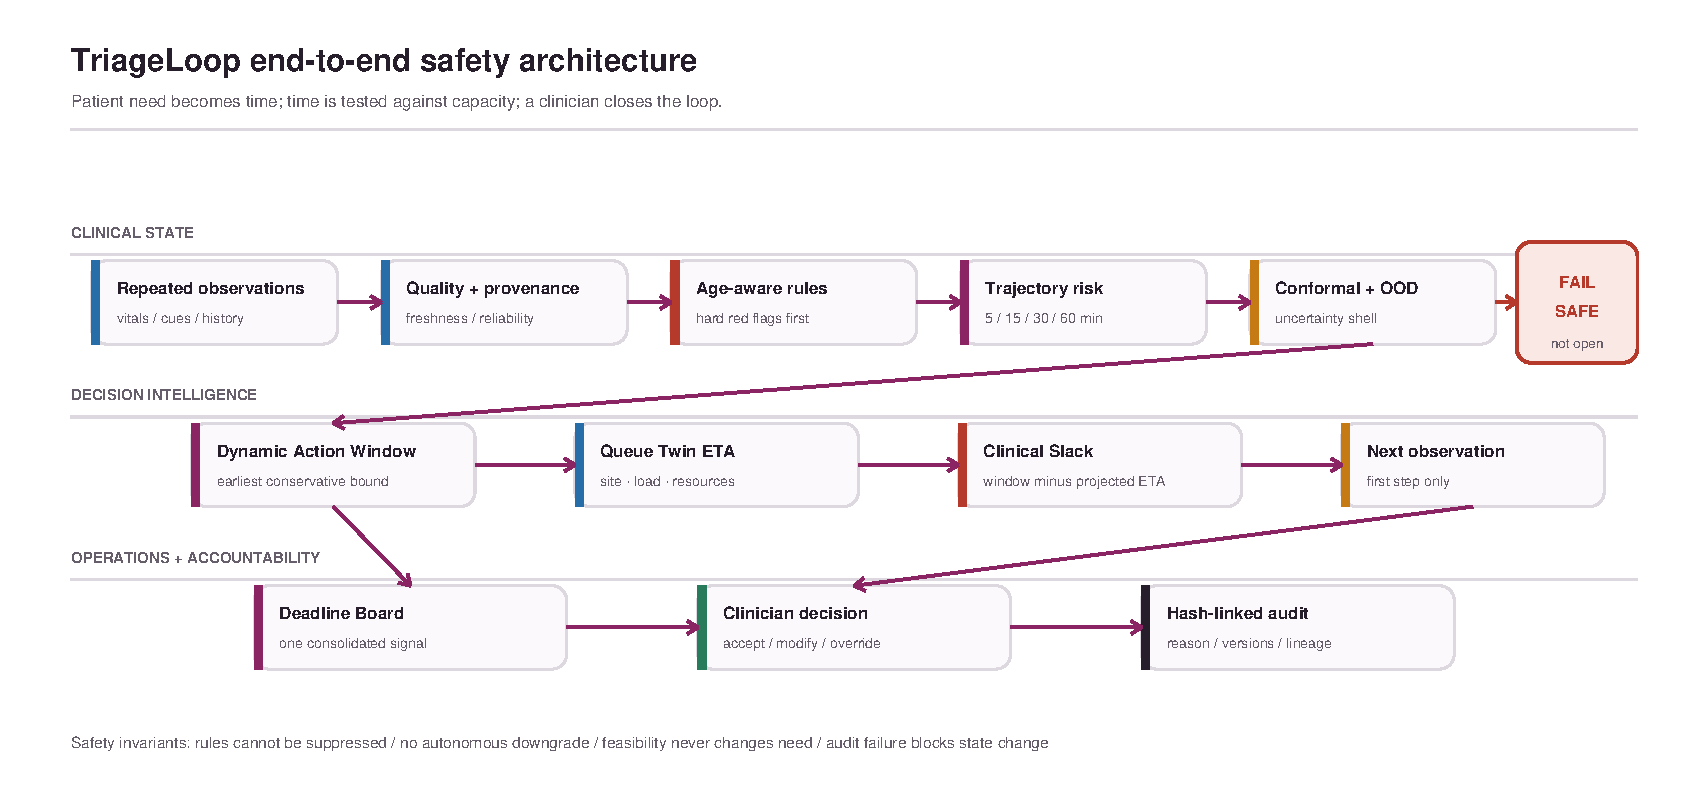
\includegraphics[width=0.97\linewidth]{figures/system_architecture.pdf}
\captionof{figure}[System architecture]{\textbf{SYSTEM ARCHITECTURE.} End-to-end layers, feedback paths and safety invariants. Clinical need is calculated before operational feasibility.}
\label{fig:architecture}
\end{center}
\vspace*{\fill}
\end{landscape}
\clearpage

\begin{center}
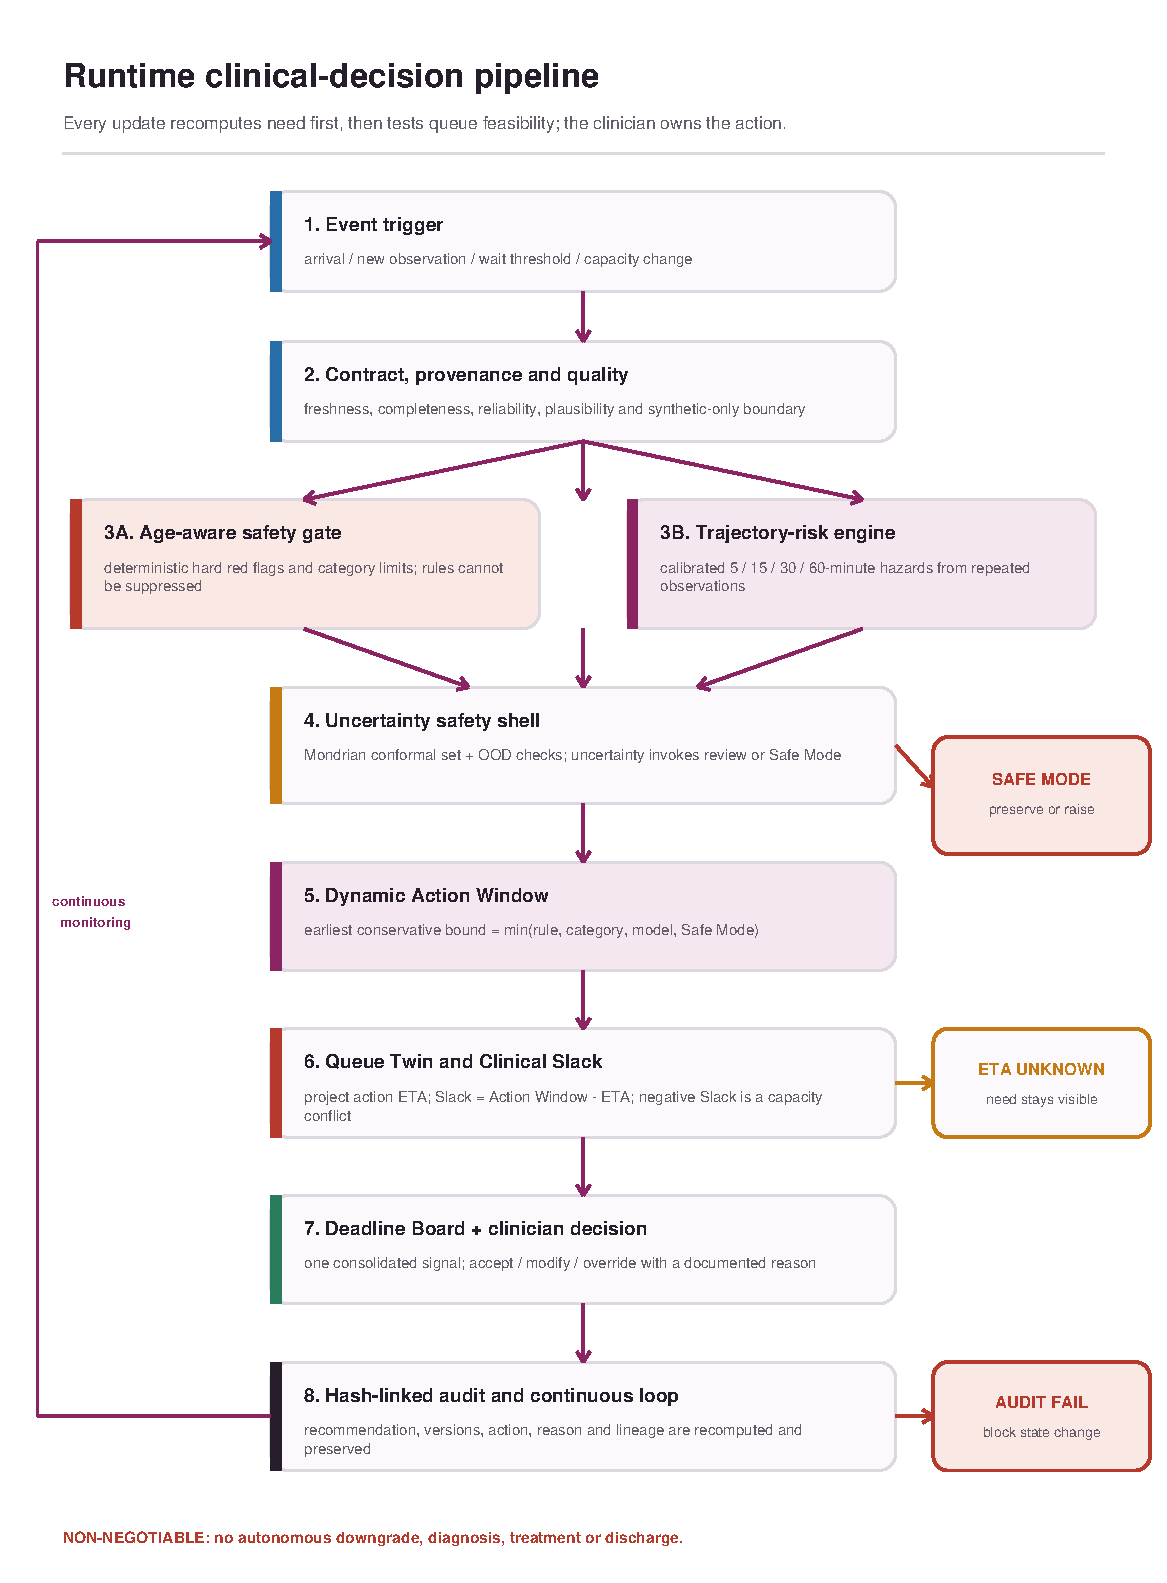
\includegraphics[height=0.80\textheight,keepaspectratio]{figures/runtime_pipeline.pdf}
\captionof{figure}[Runtime decision pipeline]{\textbf{RUNTIME PIPELINE.} Event-to-action flow for every arrival, new observation, elapsed-wait trigger or capacity change.}
\label{fig:runtimepipeline}
\end{center}
\clearpage

\finding{\textbf{Central contribution.} TriageLoop does not claim ``AI triage'' as novel. Its defensible contribution is a coherent waiting-room control loop in which repeated-observation risk constrains a conservative deadline, uncertainty invokes a specific safe response, a Queue Twin tests feasibility without rewriting clinical need, and a clinician closes an auditable loop.}

\subsection{Evidence snapshot}

\begin{table}[H]
\centering
\caption{Release-candidate evidence summary. Every quantitative performance result is synthetic or simulated.}
\begin{tabularx}{\textwidth}{@{}L{42mm}L{43mm}Y@{}}
\toprule
Evidence unit & Result & Interpretation boundary \\
\midrule
Trajectory model & Test recall 0.902-0.975; stress recall 0.891-0.982 across four horizons & Internal consistency on generated cohorts; not clinical accuracy \\
Periodic comparator & 17.7\% to 14.1\% Action Window misses; 20.5\% relative reduction & 1,200 paired synthetic policy shifts at 3x load \\
Response sensitivity & 12.8\% / 13.0\% / 24.1\% relative reductions at 10 / 20 / 30 minutes & Post-verification robustness analysis; only 30 minutes exceeds 20\% \\
NBO hypothesis & 87.5\% fewer observations, but -7.1 percentage-point critical recall & Failed safety gate; feature demoted to first-step guidance \\
External plausibility & 63,163 open MIMIC-IV demo measurements across six mapped vital fields & Input scale only; adult hospital/ICU demo, not ED transfer \\
Engineering assurance & 73/73 Python tests; type-check and optimized web build pass & Prototype verification; not certification \\
\bottomrule
\end{tabularx}
\end{table}

\section{Problem Definition and Official-Brief Coverage}

\subsection{The waiting-room failure mode}

The official PatientTriage.ai brief asks for an assistant that helps staff prioritize and route arriving patients without replacing clinical judgment, while handling age variation, incomplete information, asymmetric under-triage cost, explainability under time pressure, surge behavior, reassessment of waiting patients, override, audit, protection of patient data, and cross-hospital variability \cite{accenturebrief}. The minimum demonstration requires at least 15-20 simulated records, an ambiguous presentation, a pediatric or geriatric case, a zero-history patient, a 3x surge, explicit uncertainty, and a clinician override with its log.

A static arrival score does not fully address that specification. After intake, three coupled processes continue:

\begin{itemize}
  \item the patient's observed state evolves;
  \item evidence quality changes as new measurements appear or become stale;
  \item capacity and queue position change as arrivals and service completions occur.
\end{itemize}

TriageLoop treats the waiting room as a closed-loop safety-control problem. It does not claim to solve ED crowding or create resources. It makes the mismatch between patient-specific need and available capacity explicit soon enough for a clinician or charge nurse to act.

\subsection{Requirement-to-mechanism traceability}

\begin{longtable}{@{}L{37mm}L{54mm}L{65mm}@{}}
\caption{Official problem-statement coverage and implemented evidence.}\label{tab:pscoverage}\\
\toprule
Official complexity / expectation & TriageLoop mechanism & Implemented evidence \\
\midrule
\endfirsthead
\toprule
Official complexity / expectation & TriageLoop mechanism & Implemented evidence \\
\midrule
\endhead
Ambiguous and overlapping symptoms & Multimodal structured state, conformal prediction sets, Safe Mode, first-step NBO & Curated ambiguity scenarios; uncertainty visible in board and inspector \\
Age-specific thresholds & Pediatric/adult/geriatric stratification; deterministic age-aware safety rules & Rule catalogue, subgroup evaluation, pediatric and geriatric fixtures \\
Inconsistent intake data and zero history & Strict provenance, completeness/reliability score, freshness and plausibility checks & Zero-history contract test; missing/stale/implausible Safe Mode scenarios \\
Explainable decisions within seconds & Action-first explanation: what changed, why it matters, reliability, next action & Persistent patient inspector; corrected observed-positive model factors \\
Asymmetric under-/over-triage cost & 5:1, 10:1 and 20:1 threshold sweeps; 10:1 selected subject to recall gate & Low operating thresholds, recall-first selection, no autonomous downgrade \\
Different hospitals and staffing & Configured community, regional, and urban/trauma site profiles & 100/300/550 visits-day assumptions; baseline and 3x simulations \\
Reviewable and overridable recommendation & Accept, modify, override; reason required for material divergence & Browser-verified override and audit receipt \\
Integration maturity varies & Versioned JSON contracts, manual synthetic intake, FHIR-like boundary, SSE with fallbacks & Strict intake endpoint, schema tests, local API and proxy layer \\
Waiting-patient monitoring & Repeat observations trigger recomputation; absolute bounds age with waiting time & Deterioration event promotes P-0009 and produces -8 minutes Slack \\
Safe-wait threshold breach & Category bound and Action Window expire independently of new model output & Queue aging and capacity-conflict scenario tests \\
Patient-data protection & Synthetic-only contract, pseudonymous IDs, minimization, narrow CORS and headers & Direct name rejected; secrets/raw data/database ignored; India governance baseline \\
Adoption and alert fatigue & One consolidated current action per patient; measured alert denominators; degraded mode & 0.86-1.12 signals/waiting-patient-hour during surge; Community warning retained \\
15-20 simulated patients & Twelve-patient live board plus 28 curated fixtures and 10,000 generated encounters & Automated count/coverage tests and deterministic demo reset \\
3x surge & Queue Twin with site/load configuration and scenario switch & 1,800 original and 1,200 stronger-comparator policy shifts \\
Explicit confidence & Horizon risks, conformal set, uncertainty state, OOD, abstention and quality & Recommendation contract and live inspector \\
Clinician override and log & Reasoned state transition plus hash-linked event & Five-event live chain; tamper detection test \\
\bottomrule
\end{longtable}

\section{Research Lineage and Differentiation}

\subsection{Clinical and machine-learning foundations}

Repeated measurements can carry information that a single arrival observation cannot. A prospective ED study reported that repeated vital-sign measurements better identified deterioration than admission values alone in its infection/sepsis cohort \cite{quinten2018}. A later systematic review found potential added value in vital-sign trends but also low-certainty and sparse evidence, a boundary that argues against overstating transferability \cite{brekke2019}. These findings motivate longitudinal inputs; they do not validate TriageLoop.

Time-varying deterioration modeling and prognosis-informed prioritization provide adjacent methodological precedent \cite{timevarying2026,traumaranking2023}. TriageLoop adopts discrete-time horizon risk because the output can be calibrated, inspected, and translated into bounded action times. It does not use an LLM in the quantitative clinical path.

Uncertainty is represented explicitly because a score without a reliability state would conflict with the brief. Conformal prediction offers a distribution-free finite-sample framework under exchangeability assumptions \cite{angelopoulos2023}; a 2025 ED disposition study demonstrated the operational ``I don't know'' pattern with conformal prediction \cite{abdulai2025}. TriageLoop uses class-conditional prediction sets so rare critical cases are not hidden by aggregate coverage.

\subsection{Cross-domain transfer}

Three mechanisms are deliberately borrowed from outside conventional triage dashboards:

\begin{enumerate}
  \item \textbf{Clinical deadline from prognostics.} Remaining Useful Life estimates time remaining before an equipment state becomes unacceptable \cite{nasaRUL}. TriageLoop translates the intuition, not the literal estimator, into a conservative next-action window. It avoids phrases such as ``safe until'' because clinical time is not a known mechanical failure time.
  \item \textbf{Clinical Slack from real-time scheduling.} Deadline and laxity scheduling asks how much scheduling freedom remains before a deadline is missed \cite{liu1973}. TriageLoop computes Slack as patient-specific time requirement minus projected action time, while retaining deterministic category and rule precedence.
  \item \textbf{Next Best Observation from active feature acquisition.} Active acquisition asks which costly feature would most improve a case-specific decision \cite{ibmafa}. The prototype restricts candidate actions to low-burden observations and questions; it does not autonomously order treatment, imaging, or laboratory tests.
\end{enumerate}

\subsection{Prior art and novelty boundary}

Dynamic clinical queues, continuous reassessment, and AI-supported triage all have precedent. The closest identified 2026 India-focused OPD work combines LLM-based severity prediction, urgency-drift detection, longitudinal memory, and adaptive queue optimization in simulation \cite{gupta2026}. TriageLoop therefore does not claim ``world first,'' patent novelty, or ownership of dynamic queues.

The narrower distinction is the system-level composition shown in Figure~\ref{fig:architecture}: an ED waiting-room workflow; deterministic rules before ML; no LLM in the numerical path; calibrated multi-horizon trajectory risk; conformal/OOD Safe Mode; a conservative Action Window; explicit capacity feasibility through Slack; NBO constrained by a failed safety gate; no autonomous downgrade; and clinician-linked audit. Novelty is claimed as a design recomposition and working prototype, not as clinical validation.

\begin{figure}[H]
\centering
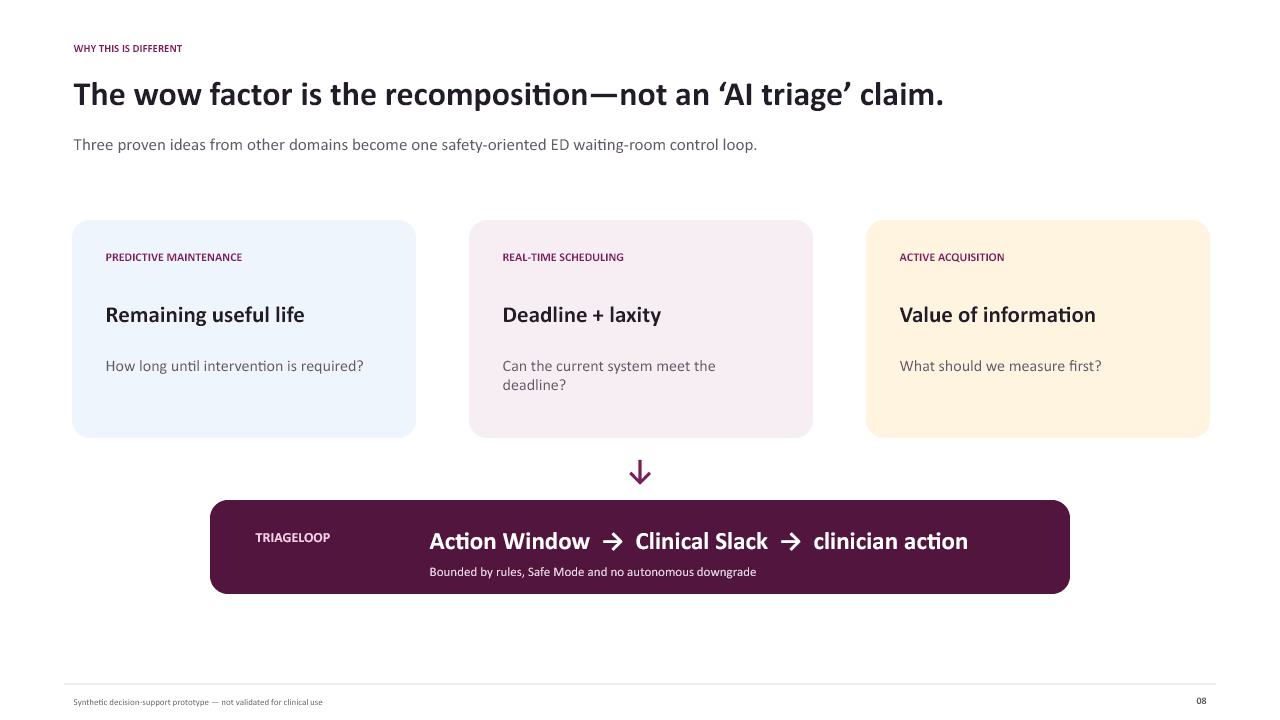
\includegraphics[width=0.95\textwidth]{../submission/visuals/03-unique-recomposition.png}
\caption{The differentiation claim is a recomposition of established ideas, not invention of the individual components.}
\end{figure}

\section{Safety Contract and System Invariants}

The clinical safety contract was locked before implementation. Its purpose is to define what the prototype may never do, independent of model performance.

\begin{table}[H]
\centering
\caption{Core safety invariants and failure behavior.}
\begin{tabularx}{\textwidth}{@{}L{40mm}Y Y@{}}
\toprule
Invariant & Normal behavior & Failure behavior \\
\midrule
Rules precede model & Hard red flags immediately constrain action & Model output cannot suppress or lengthen the rule requirement \\
No autonomous downgrade & Clinician-assigned state is preserved unless a clinician changes it & Model may recommend earlier review or promotion only \\
Uncertainty escalates & Ambiguous/OOD/poor-quality state is named and prompts reassessment & Safe Mode uses a conservative bound and specific reason \\
Need is separate from capacity & Action Window remains a clinical requirement & Queue failure removes ETA/Slack confidence, not the patient deadline \\
Human authority is explicit & Accept, modify, and override are available & Modify/override requires reason; persistence failure blocks the digital action \\
Audit is verified, not asserted & Every event stores previous hash and event hash & Integrity endpoint recomputes all links and reports first broken event \\
Degraded mode is honest & Live state and controls are available only with service connection & UI labels last-verified context, suppresses estimates, disables actions, and directs downtime workflow \\
\bottomrule
\end{tabularx}
\end{table}

When multiple triggers occur, the system does not emit competing actions. It selects the most conservative action and preserves all contributing reasons. A compound fixture combines a hard red flag, Safe Mode, and an exceeded wait threshold to verify this behavior.

The prototype's deterministic thresholds are conservative demonstration rules, not a deployable clinical protocol. Pediatric separation is motivated by WHO's separate child and adult/adolescent facility triage tools \cite{whotriage}; geriatric handling adds frailty, comorbidity, and atypical-presentation context but still requires local clinical governance.

\section{Data Strategy and Synthetic Longitudinal Cohort}

\subsection{Why synthetic data is primary}

The competition does not require proprietary hospital data and explicitly permits realistic simplified or simulated records \cite{accenturebrief}. Synthetic generation was chosen to guarantee pediatric, geriatric, ambiguous, missing-data, zero-history, and surge cases while avoiding identifiable patient information and access delays. This choice enables reproducibility but creates the paper's largest validity threat: the model, generator, and Queue Twin originate in one project.

The paper therefore distinguishes three evidence classes:

\begin{itemize}
  \item \textbf{curated scenario evidence} verifies required and adversarial behavior;
  \item \textbf{synthetic statistical evidence} checks internal model and queue hypotheses under declared assumptions;
  \item \textbf{external plausibility evidence} checks only whether input scales are grossly disconnected from an open reference.
\end{itemize}

\subsection{Population and split}

The locked generator uses seed \code{20260821} to create 10,000 longitudinal encounters and 30,020 time-indexed snapshots. The final snapshot allocation is 17,114 train, 5,685 validation, 5,708 untouched test, and 1,513 deliberate stress snapshots. Splits are patient-level. Validation is internally separated so probability calibration and conformal/threshold selection do not reuse the same examples.

History availability is approximately balanced: 4,921 encounters have some prior history and 5,079 have none. The generated population spans pediatric, adult, and geriatric bands; the stress cohort changes age mix, missingness, prevalence, arrival load, and measurement noise.

\subsection{Observation contract and temporal leakage controls}

Each patient state contains a pseudonymous identifier, age, sex at birth, complaint, symptoms, observed cues, history availability, clinician state, and an ordered observation series. Every observation records time, source, vital values, completeness, reliability, and synthetic provenance. Future observations and hidden deterioration labels are excluded from features at prediction time.

Forty-four standardized/imputed features include current values, deltas, missing indicators, age bands, history state, clinician level, elapsed wait, data quality, and bounded text-cue flags. The feature ``number of observations'' was removed after audit because it could encode workflow intensity rather than physiology. This is an example of process-derived leakage: a model can appear predictive by learning how often staff already chose to measure a patient.

\clearpage
\begin{landscape}
\thispagestyle{fancy}
\vspace*{\fill}
\begin{center}
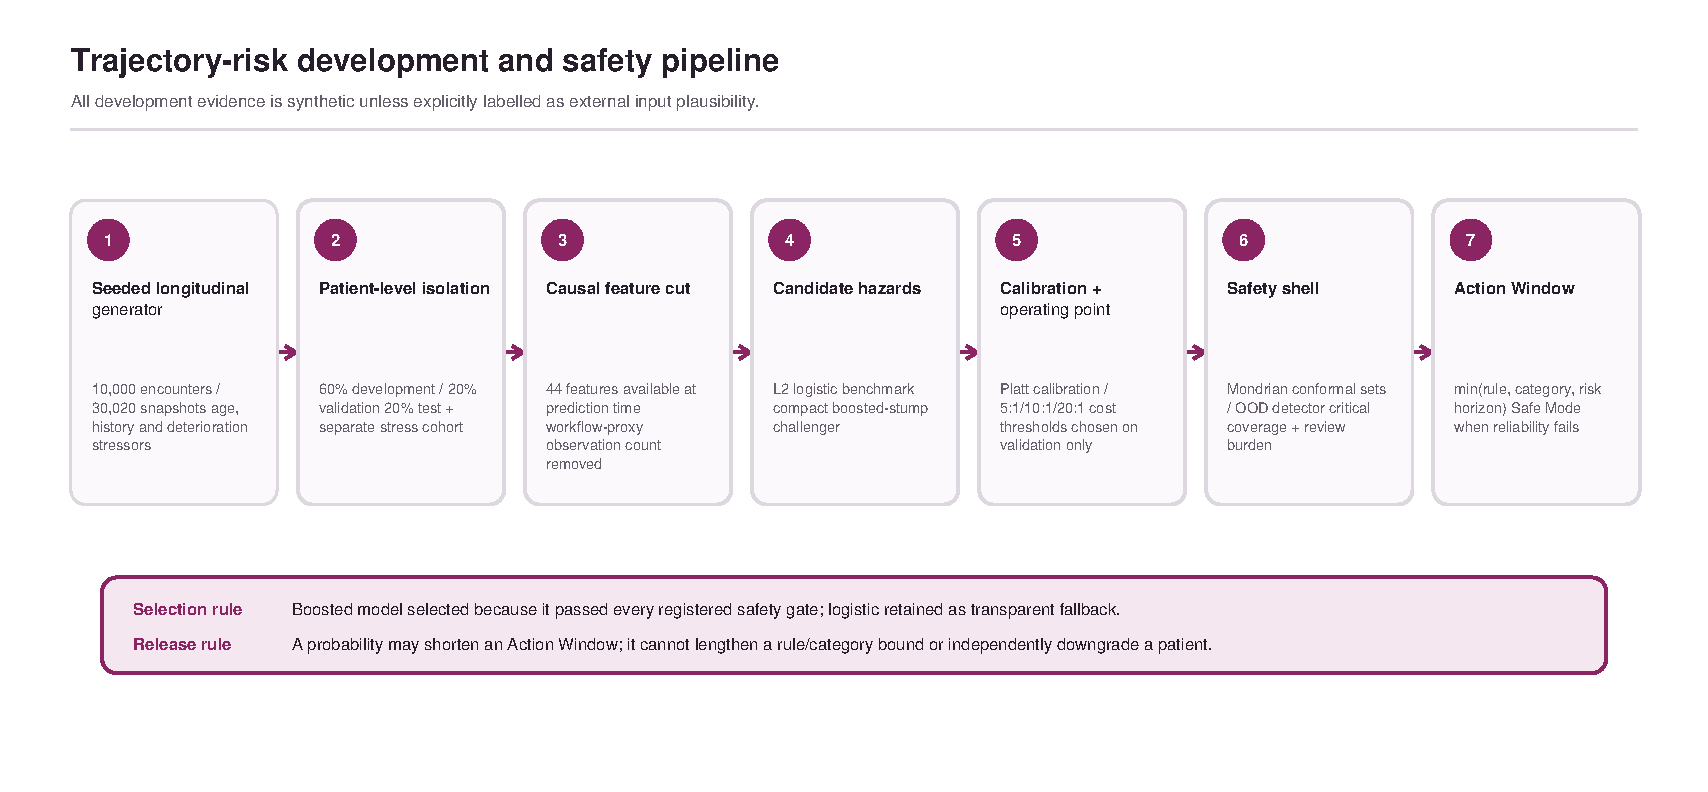
\includegraphics[width=0.97\linewidth]{figures/ml_pipeline.pdf}
\captionof{figure}[ML development and validation pipeline]{\textbf{ML DEVELOPMENT AND VALIDATION PIPELINE.} Data generation, patient-level isolation, leakage control, candidate comparison, calibration, uncertainty gates and release rule.}
\label{fig:mlpipeline}
\end{center}
\vspace*{\fill}
\end{landscape}
\clearpage

\subsection{Curated cases}

Twenty-eight deterministic fixtures cover ambiguous presentations, pediatric and geriatric states, no-history intake, missing and stale data, worsening vital signs, hard-rule/model conflict, compound triggers, multiple critical patients, NBO unavailability, and override/audit behavior. Twelve of these appear on the live board to keep the jury demonstration readable while the full set remains in automated tests.

\section{Trajectory-Risk and Uncertainty Methodology}

\subsection{Prediction target}

For each snapshot $x_{i,t}$, the model estimates simulated need for urgent clinical escalation within horizons $h\in\{5,15,30,60\}$ minutes:

\begin{equation}
p_{i,t,h}=P(T_i \le t+h\mid T_i>t, x_{i,t}).
\end{equation}

The generated composite can represent a resuscitation-level vital abnormality, urgent senior review, monitored-care requirement, or treatment-space escalation. It is not time to death, a diagnosis, or a promise of safety until a particular minute. Horizon probabilities are monotonized after calibration so longer horizons do not report less cumulative risk than shorter ones.

\subsection{Candidates and model selection}

The primary benchmark is an L2-regularized discrete-time logistic hazard model. The challenger is a compact gradient-boosted ensemble of shallow logistic decision stumps. Both use the same feature transformer and Platt calibration. AUROC alone is prohibited as a selection criterion. The challenger may win only through a meaningful safety/calibration advantage without unacceptable subgroup or explanation burden.

The boosted model was selected by a registered gate override. The logistic benchmark had slightly better mean test Brier score (0.0476 versus 0.0498), but failed short-horizon/stress gates after removal of the workflow-proxy feature. The boosted model passed every registered horizon-level recall, in-distribution ECE, and critical-class conformal-coverage gate. Its mean stress recall was 0.941 versus 0.862 for logistic.

\begin{table}[H]
\centering
\caption{Selected boosted-hazard performance by horizon on synthetic cohorts.}
\small
\begin{tabularx}{\textwidth}{@{}L{15mm}*{6}{>{\centering\arraybackslash}X}@{}}
\toprule
Horizon & Test recall & Stress recall & Test ECE & Test critical coverage & Stress critical coverage & Test positive rate \\
\midrule
5 min  & 0.914 & 0.891 & 0.003 & 0.973 & 0.977 & 0.080 \\
15 min & 0.902 & 0.923 & 0.008 & 0.902 & 0.923 & 0.267 \\
30 min & 0.975 & 0.982 & 0.016 & 0.975 & 0.982 & 0.545 \\
60 min & 0.949 & 0.968 & 0.026 & 0.949 & 0.968 & 0.523 \\
\bottomrule
\end{tabularx}
\end{table}

\begin{figure}[H]
\centering
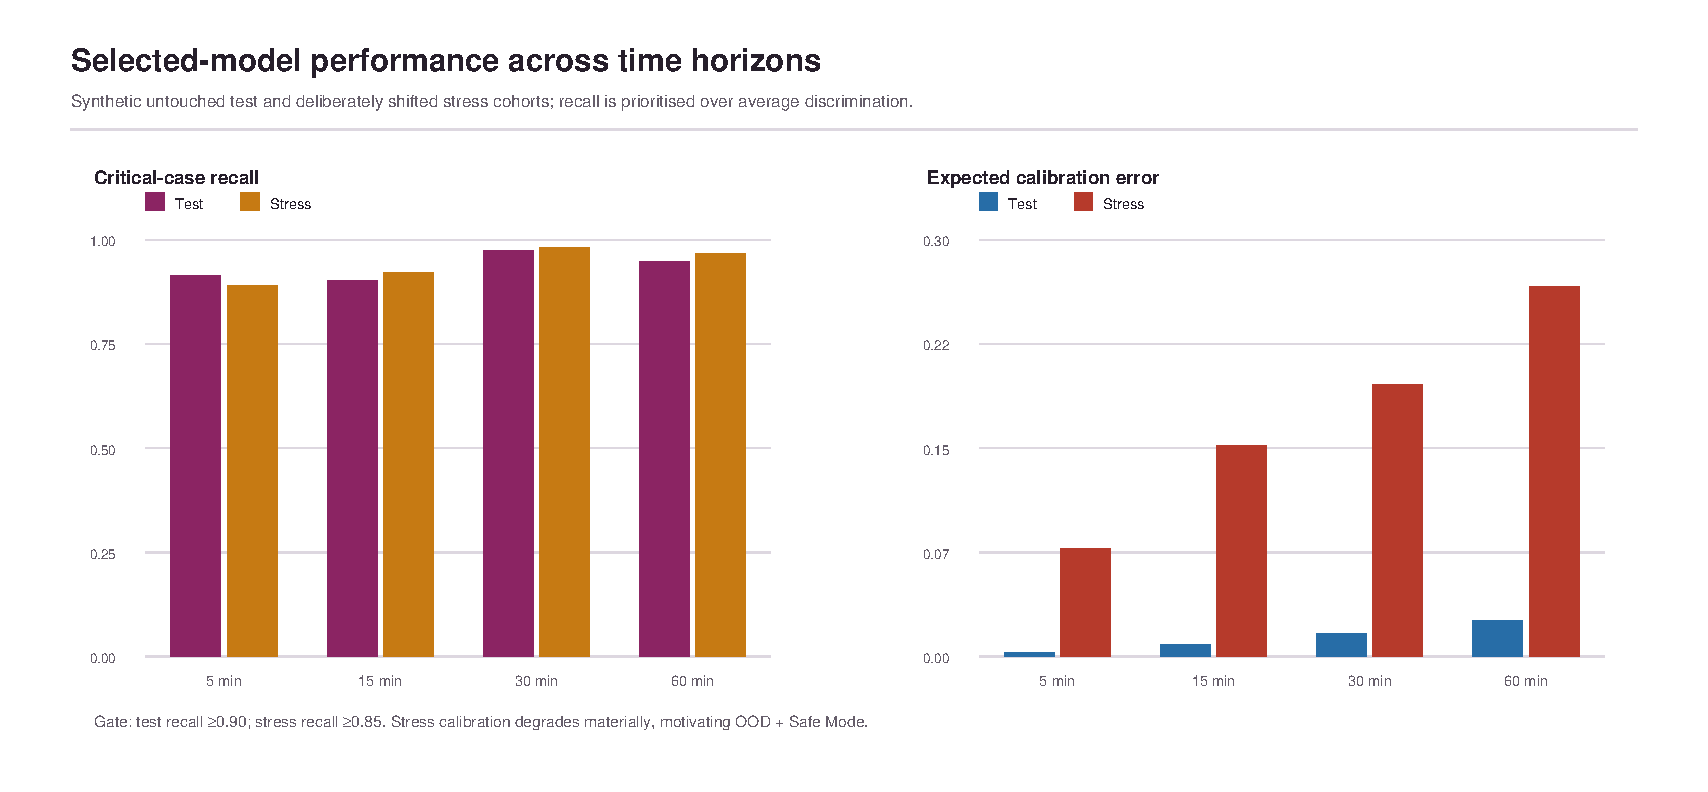
\includegraphics[width=\textwidth]{figures/model_results.pdf}
\caption{Selected-model recall and calibration by horizon. Stress ECE deterioration motivates explicit shift handling.}
\label{fig:modelresults}
\end{figure}

\subsection{Asymmetric decision cost}

Thresholds are selected on validation data at cost ratios $C_{FN}:C_{FP}\in\{5:1,10:1,20:1\}$ with a minimum validation recall constraint. The chosen prototype setting is 10:1:

\begin{equation}
\tau_h^*=\arg\min_{\tau}\left(C_{FN}\,FN_h(\tau)+C_{FP}\,FP_h(\tau)\right)
\quad\text{subject to}\quad \mathrm{Recall}_h(\tau)\ge 0.90.
\end{equation}

The resulting thresholds are 0.4100, 0.0393, 0.0600, and 0.1225 at 5/15/30/60 minutes. The low 15- and 30-minute thresholds make the intended escalation bias visible. They also increase review workload, so the product consolidates multiple model/rule states into one current patient action and reports alert denominators rather than calling the burden manageable.

\subsection{Conformal sets, OOD, and Safe Mode}

The prototype uses 90\% nominal class-conditional (Mondrian) conformal prediction sets. For class $y$ and nonconformity score $s(x,y)$, the prediction set is

\begin{equation}
\Gamma_{\alpha}(x)=\{y:s(x,y)\le q_{y,1-\alpha}\},
\end{equation}

where $q_{y,1-\alpha}$ is calculated from the isolated conformal calibration subset. A singleton set communicates a bounded prediction; a set containing both labels is ambiguous; an empty or materially ambiguous near-term set triggers review. Coverage is evaluated separately for the critical class because overall coverage could conceal rare-class failure.

A feature-space OOD detector flags 1.1\% of test snapshots and 18.2\% of stress snapshots. Missing, stale, implausible, low-reliability, OOD, or materially ambiguous near-term states activate Safe Mode. Safe Mode does not invent a more precise probability. It recommends conservative review, states why the numerical path is unreliable, and prevents automated downgrade.

\subsection{Explanation contract}

The nurse-facing explanation answers four questions: what action is recommended, by when, what changed, and why the system trusts or distrusts its estimate. Local stump contributions are translated only when they are positive urgency drivers grounded in observed values. A TL-06.5 review found that an absent binary feature could receive a mathematically valid negative centered contribution and be verbalized as if the finding were present. The numerical score was unchanged, but the sentence was clinically backward. The renderer was corrected to admit only observed positive drivers, and a regression test now checks the deteriorating P-0009 case.

\section{Dynamic Action Window and Next Best Observation}

\subsection{Action Window derivation}

The Action Window is a conservative interval by which the next specified action is recommended. For patient $i$ at time $t$,

\begin{equation}
W_i(t)=\min\left[
W_{\mathrm{hard},i}(t),
\max(0,W_{\mathrm{cat},i}-e_i(t)),
\inf\{h:p_{i,t,h}\ge\tau_h\},
W_{\mathrm{safe},i}(t)
\right],
\end{equation}

where $e_i(t)$ is elapsed wait, the category term is an upper bound, the model term is the earliest calibrated threshold crossing, and Safe Mode contributes a five-minute maximum in the prototype. Missing terms are treated as $+\infty$. A hard red flag yields immediate review. The interface says ``recommended within''; it never says ``safe until.''

This design converts a probability vector into a workflow constraint without pretending that the model predicts an exact deterioration moment. It also makes waiting-time aging explicit: even without a new observation, a category-bound window shrinks as elapsed time increases.

\subsection{Next Best Observation}

When uncertainty is decision-relevant and no hard rule already determines the action, the system ranks a clinician-approved catalogue containing repeat SpO2, respiratory rate, heart rate, blood pressure, temperature, mental status/GCS, pain, and symptom-onset clarification. A conceptual value function is

\begin{equation}
o^*=\arg\max_{o\in\mathcal O}
\frac{\mathbb{E}[\Delta D\mid o]}{t_o+\lambda b_o},
\end{equation}

where $\Delta D$ is estimated decision impact, $t_o$ is typical acquisition time, and $b_o$ is burden. The implementation combines model feature importance, proximity to the decision threshold, and quality defects. Candidate observations are suggestions only; no treatment, laboratory, or imaging order is generated.

The predeclared gate required at least 25\% fewer observations with no more than two percentage points of operational critical-recall loss versus an eight-observation bundle. The one-observation policy failed decisively on 4,317 eligible snapshots: recall fell from 0.959 to 0.888. A four-observation adaptive fallback passed the test split but failed independent stress confirmation. Selecting a five-observation bundle after viewing stress would be post-hoc tuning, so it was rejected.

\begin{figure}[H]
\centering
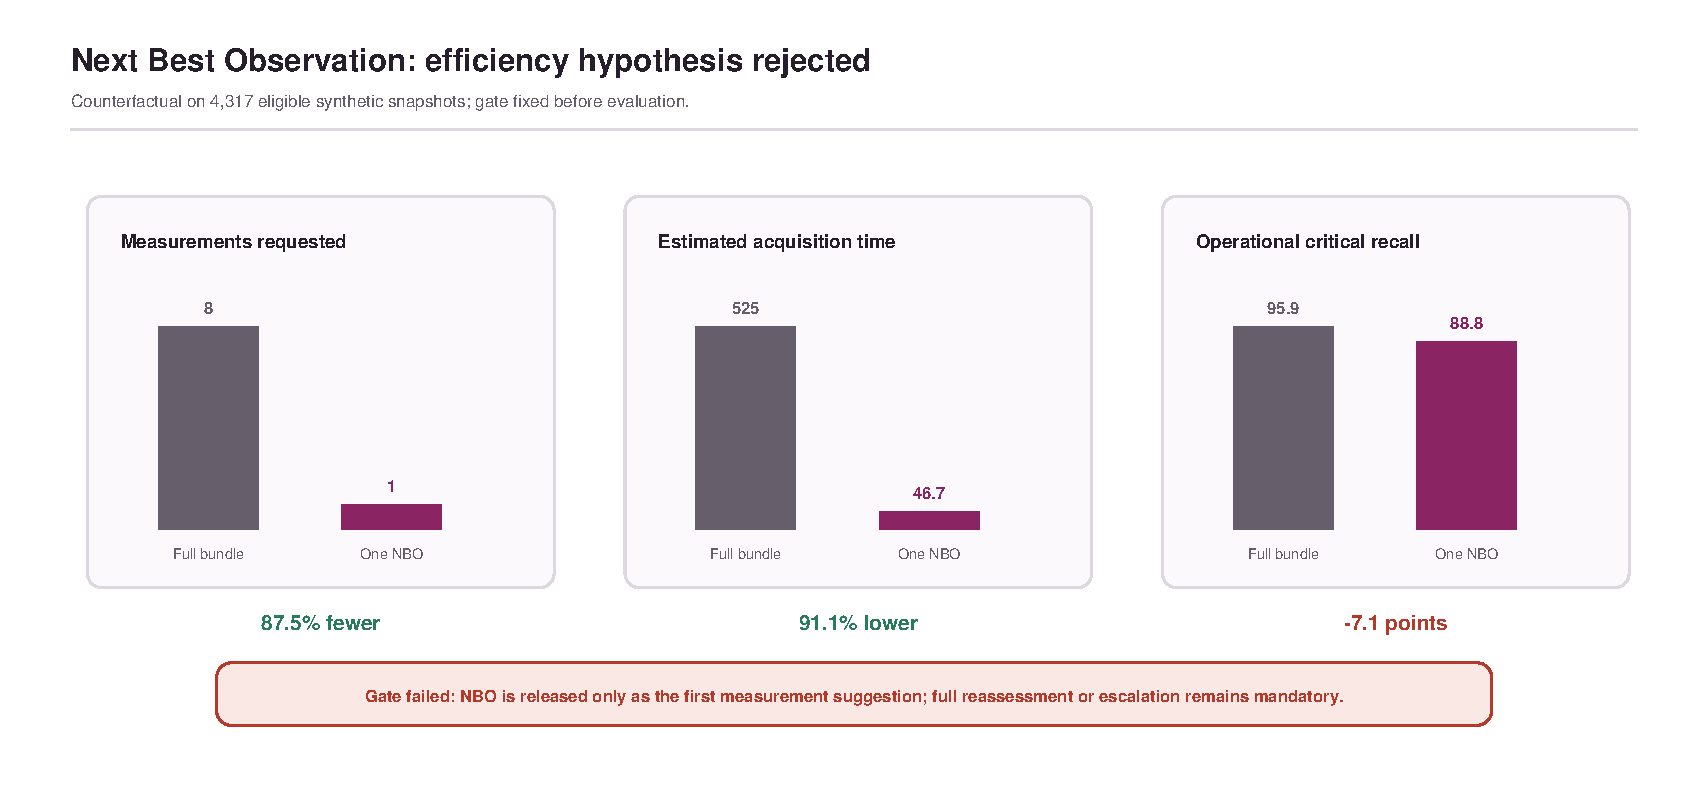
\includegraphics[width=\textwidth]{figures/nbo_tradeoff.pdf}
\caption{NBO gate outcome. The efficiency gain did not preserve the fixed safety boundary.}
\label{fig:nbo}
\end{figure}

\finding{\textbf{Release consequence.} The product may show NBO as the first measurement suggestion. If the measurement is unavailable, uncertainty persists, or clinical concern remains, the required behavior is full reassessment or escalation. No workload-reduction or recall-preservation claim is permitted.}

\section{Queue Twin, Clinical Slack, and Scheduling Policy}

\subsection{Queue Twin}

The Queue Twin is a seeded discrete-event simulator and live projection layer. It estimates time to the next clinical action using current queue state, site profile, load, clinician capacity, reassessment staff, monitored spaces, service-time distributions, and priority policy. It is not a staffing optimizer and is not calibrated to a real hospital.

The original registered matrix contains three policies, three sites, two loads, and 100 paired replications per cell: 1,800 policy shifts. TL-05 added a stronger two-policy matrix: fixed 15-minute periodic re-triage versus TriageLoop across the same sites, loads, and replications, totaling 1,200 policy shifts.

\subsection{Clinical Slack}

For patient $i$,

\begin{equation}
S_i(t)=W_i(t)-\widehat{\eta}_i(t).
\end{equation}

$S_i>0$ means projected capacity can meet the current window under the simulator's assumptions. $S_i=0$ means the deadline is due. $S_i<0$ means the current queue is projected to act after the requirement. The UI labels the latter ``Capacity conflict'' and asks for operational escalation; it does not relax the patient deadline.

The production policy is no-demotion and lexicographic. Hard rules determine immediate action. The dynamic category follows, allowing strong repeat-observation risk to promote but not autonomously demote. Absolute Action Window, calibrated risk, uncertainty, and arrival time resolve later ties. This policy was selected after pure earliest-deadline scheduling grouped excessive false-positive 30-minute windows and failed the registered gate.

\subsection{Primary queue result}

Under simulated 3x load, TriageLoop reduced Action Window misses from 17.7\% to 14.1\% versus fixed 15-minute periodic re-triage, a 20.5\% relative reduction (95\% paired-bootstrap CI 17.4\%-23.8\%). It also reduced negative-Slack minutes by 14.0\%, signal-to-action time by 15.7\%, and low-acuity P90 wait by 14.4\% in the same overall comparison.

\begin{figure}[H]
\centering
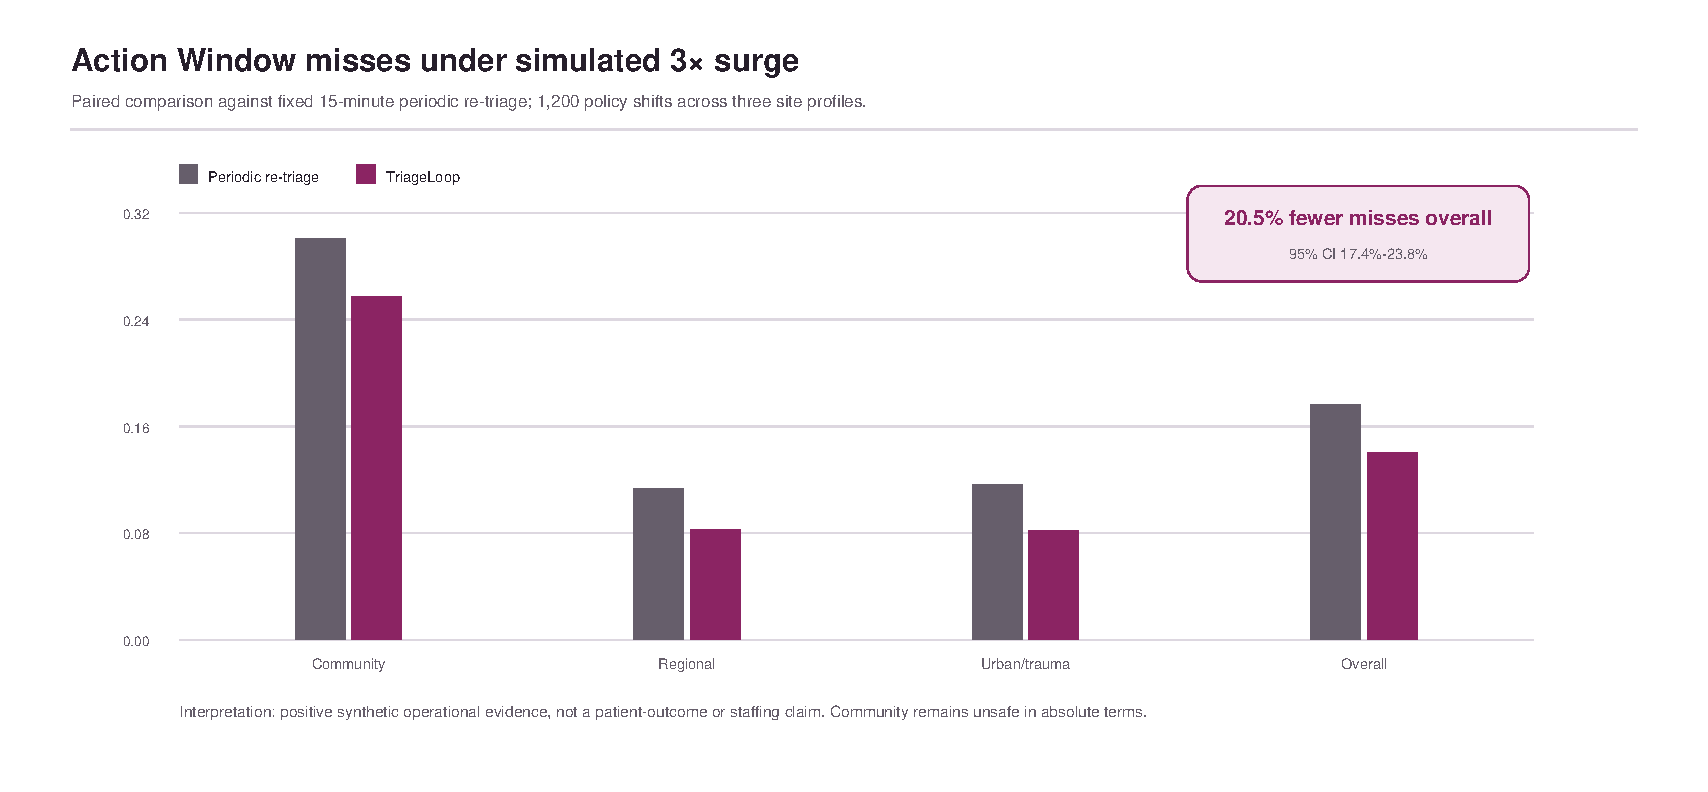
\includegraphics[width=\textwidth]{figures/queue_results.pdf}
\caption{Site and overall Action Window miss rates under simulated 3x surge.}
\label{fig:queue}
\end{figure}

The result is not uniform proof of safety. Under baseline capacity all compared policies have zero critical misses, so TriageLoop has no measurable miss-rate advantage. Community surge remains unsafe in absolute terms despite improvement. In the earlier static comparison its miss rate remains 25.7\% and critical recall 0.743. Software cannot create staff, beds, or monitored spaces; the product must keep negative Slack visible.

\subsection{Response-definition sensitivity}

The composite deterioration target includes immediate red flags and broader urgent review/monitoring/treatment escalation. The simulation therefore reports sensitivity to a 10-, 20-, and 30-minute response allowance. Against the stronger periodic comparator, relative miss-rate reductions were 12.8\%, 13.0\%, and 24.1\%, with positive paired intervals at each definition. Only the 30-minute definition exceeds 20\%. This analysis was added after TL-05 in response to independent review and is not a retroactively registered gate.

\begin{figure}[H]
\centering
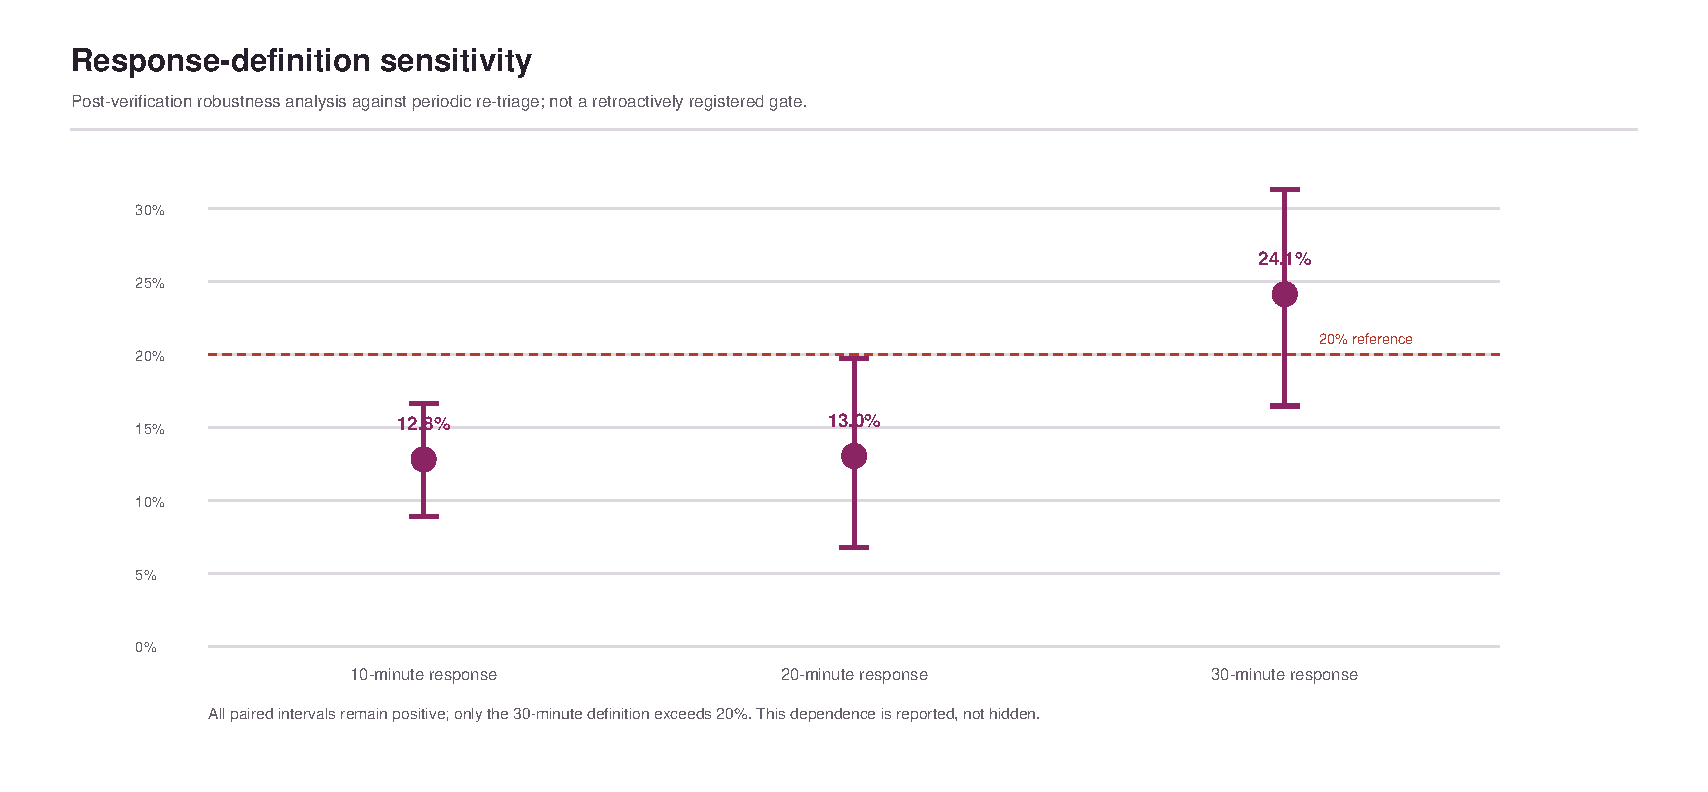
\includegraphics[width=\textwidth]{figures/response_sensitivity.pdf}
\caption{Post-verification response-definition sensitivity and paired confidence intervals.}
\label{fig:sensitivity}
\end{figure}

\subsection{Alert workload}

Signals are consolidated at patient level within each eight-hour shift. During surge, TriageLoop produces 0.86-1.12 consolidated alerts per waiting-patient-hour and 2.20-5.56 alerts per configured reassessment-nurse-hour across site profiles. Community surge is the warning case at 5.56 signals per nurse-hour under the one-nurse assumption. No ``safe workload'' threshold is claimed; real nurse time-and-motion and alert-acknowledgement studies remain external work.

\section{Software and Product Architecture}

\subsection{Deployment units}

The system is separated into a nurse-facing Next.js application, a FastAPI decision/simulation service, versioned JSON contracts, and a SQLite prototype store. The frontend never recomputes clinical logic. It calls a same-origin server proxy, which forwards to the configured API. The API owns validation, recommendation, simulation state, clinician decisions, and audit integrity.

\begin{table}[H]
\centering
\caption{Prototype deployment units and responsibilities.}
\begin{tabularx}{\textwidth}{@{}L{35mm}L{50mm}Y@{}}
\toprule
Unit & Technology & Responsibility \\
\midrule
Nurse interface & Next.js App Router / TypeScript & Deadline Board, patient inspector, Capacity, Audit, Evidence, About/resilience surfaces \\
Decision service & Python 3.12 / FastAPI & Contracts, rules, model inference, uncertainty, Action Window, manual synthetic intake, decisions \\
Operational layer & Seeded discrete-event simulation & Queue ETA, site/load scenarios, Slack, paired evaluation \\
Prototype store & SQLite & Deterministic demo state, decision state, append-only hash-linked audit events \\
Contracts & JSON Schema / Pydantic & Strict patient, recommendation, and queue snapshot boundaries \\
Container path & Docker Compose & API health-gated startup followed by standalone Next.js service \\
\bottomrule
\end{tabularx}
\end{table}

The API exposes health/configuration, demo state and reset, scenario changes, deterioration events, patient/recommendation retrieval, manual synthetic intake, decisions, audit, audit-integrity verification, evaluation artifacts, and a server-sent event stream. CORS permits only configured origins, state-changing methods are restricted, and request models reject unknown direct identifier fields.

\subsection{Product interaction model}

The primary surface is a clinical Deadline Board, not a generic analytics dashboard. Each row shows rank, pseudonymous patient, age band, complaint, current level, action, Action Window, ETA, Slack, uncertainty, and latest change. A persistent inspector follows a fixed order: recommendation; deadline/ETA/Slack; trajectory; reasons and uncertainty; first-step NBO; clinician decision.

Meaning never depends on color alone. Red is reserved for clinical urgency and capacity conflict; brand berry indicates selection and primary actions. The system targets WCAG 2.2 AA structure through one H1, skip link, labeled controls, table captions/headers, visible focus, reduced motion, and text equivalents. This is structural prototype evidence, not formal assistive-technology or nurse-usability validation.

\begin{figure}[H]
\centering
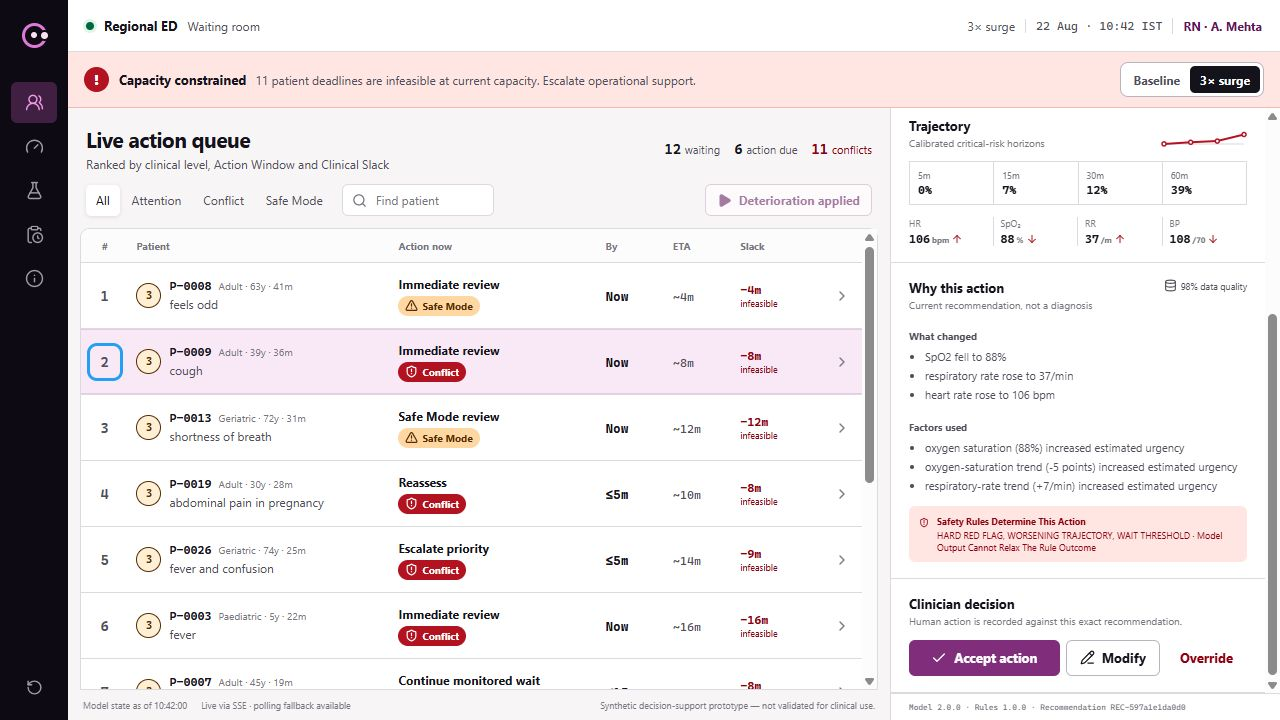
\includegraphics[width=0.96\textwidth]{../submission/visuals/product-surfaces/01-live-board-corrected.png}
\caption{Working Deadline Board after a deterioration event. The patient-level deadline and queue-level capacity conflict are shown together without collapsing them into one score.}
\label{fig:board}
\end{figure}

\begin{figure}[H]
\centering
\begin{minipage}[t]{0.49\textwidth}
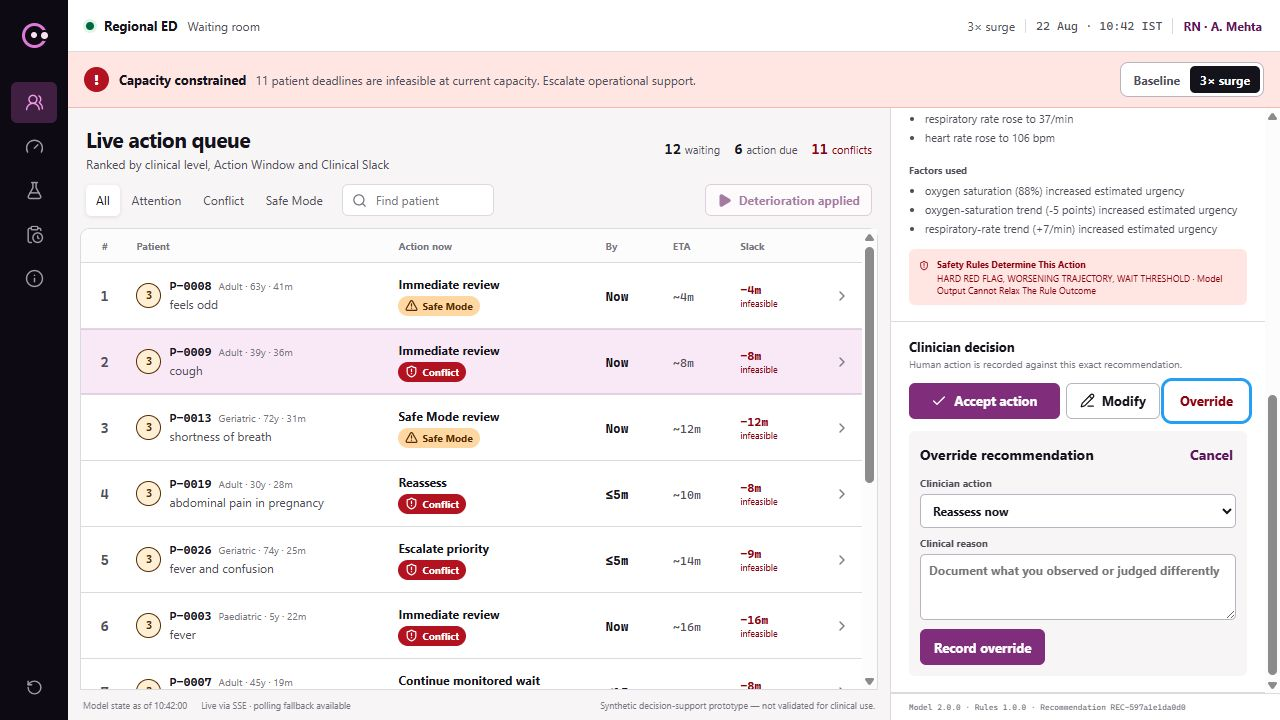
\includegraphics[width=\linewidth]{../submission/visuals/product-surfaces/02-override-mid-flow.png}
\centering\small\textbf{(a)} Reasoned clinician override.
\end{minipage}\hfill
\begin{minipage}[t]{0.49\textwidth}
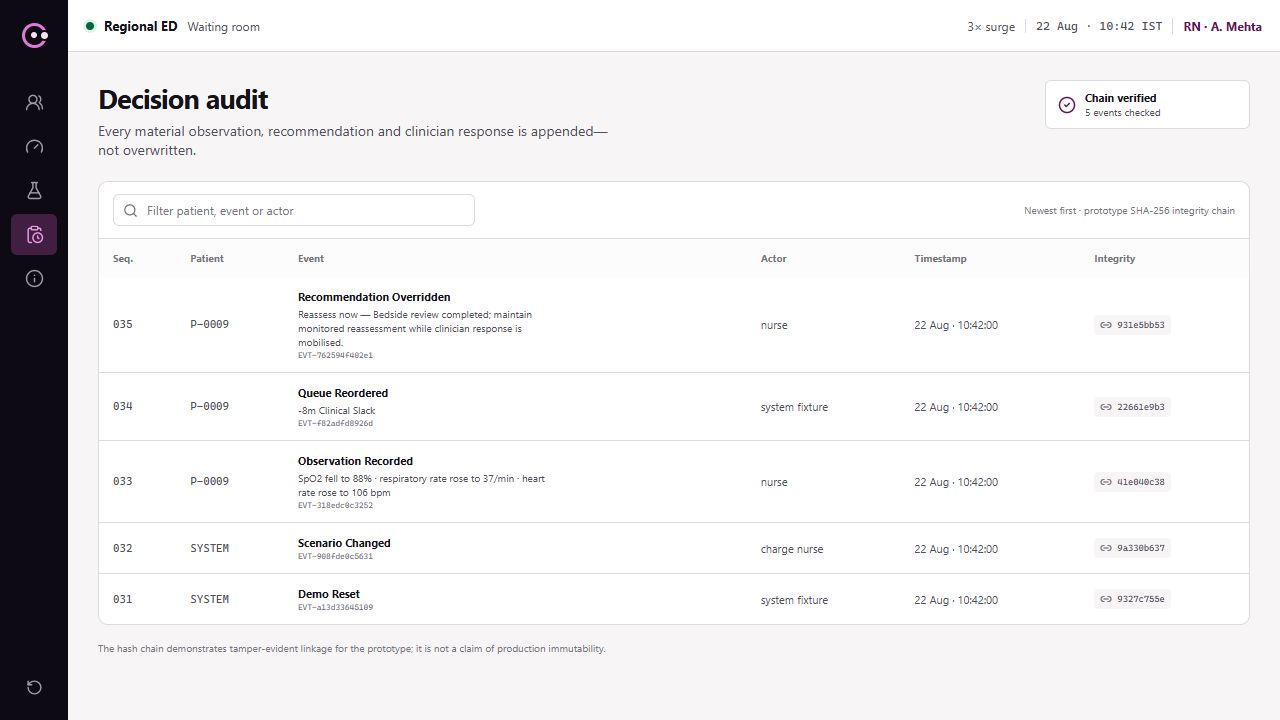
\includegraphics[width=\linewidth]{../submission/visuals/product-surfaces/03-audit-chain.png}
\centering\small\textbf{(b)} Recomputed hash-linked audit chain.
\end{minipage}
\caption{Human authority is a visible product state, not a disclaimer.}
\end{figure}

\begin{figure}[H]
\centering
\begin{minipage}[t]{0.49\textwidth}
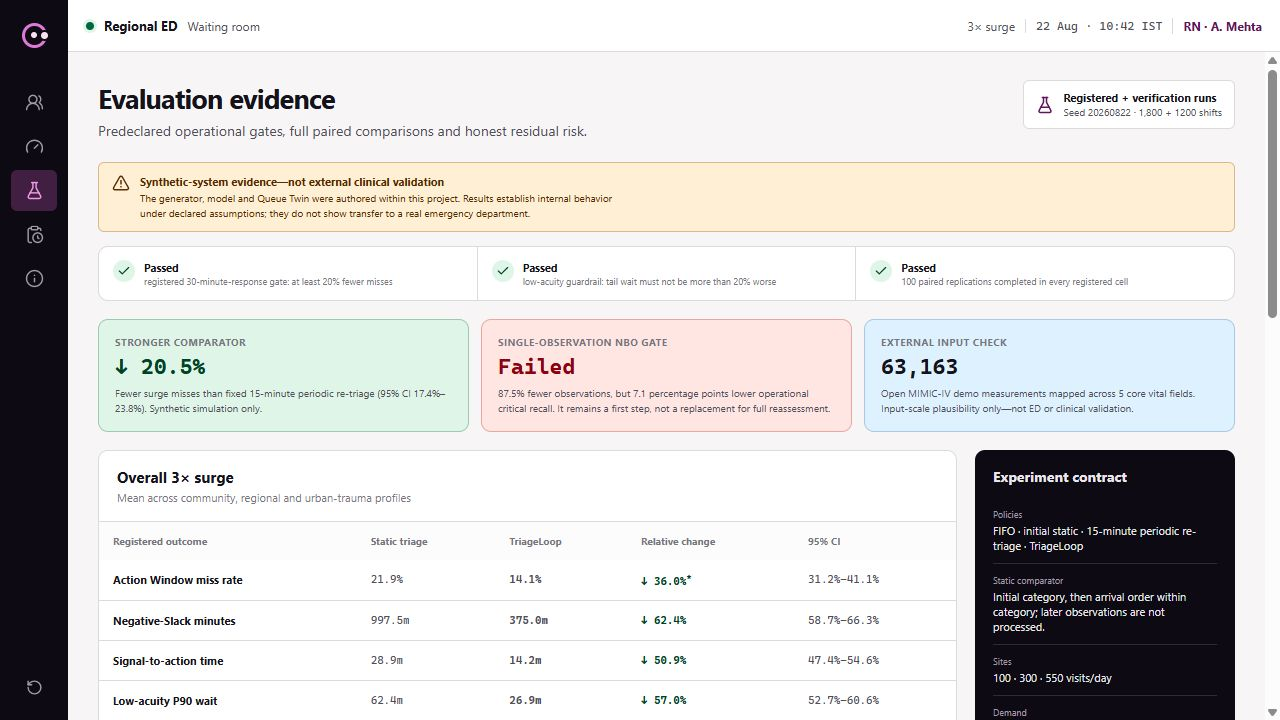
\includegraphics[width=\linewidth]{../submission/visuals/product-surfaces/04-evidence.png}
\centering\small\textbf{(a)} Evidence and limitations surface.
\end{minipage}\hfill
\begin{minipage}[t]{0.49\textwidth}
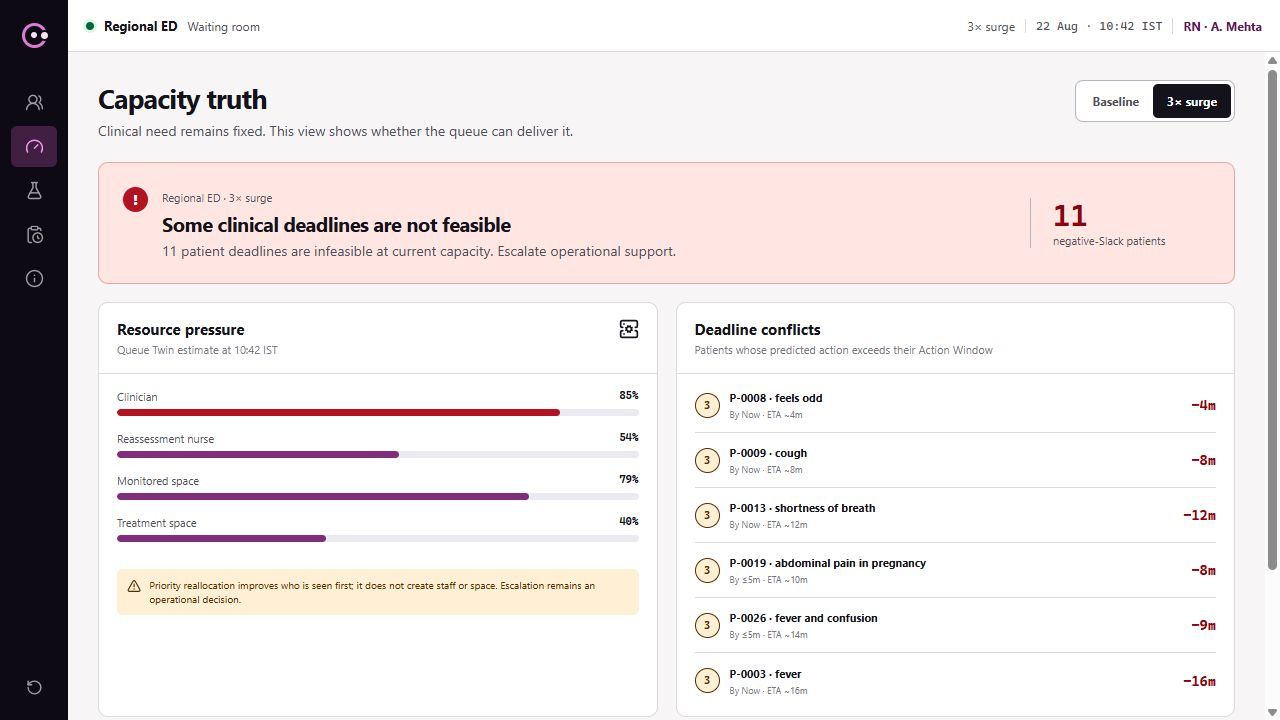
\includegraphics[width=\linewidth]{../submission/visuals/product-surfaces/05-capacity-truth.png}
\centering\small\textbf{(b)} Capacity truth under surge.
\end{minipage}
\caption{Scientific evidence and operational constraints are available from the working product.}
\end{figure}

\begin{figure}[H]
\centering
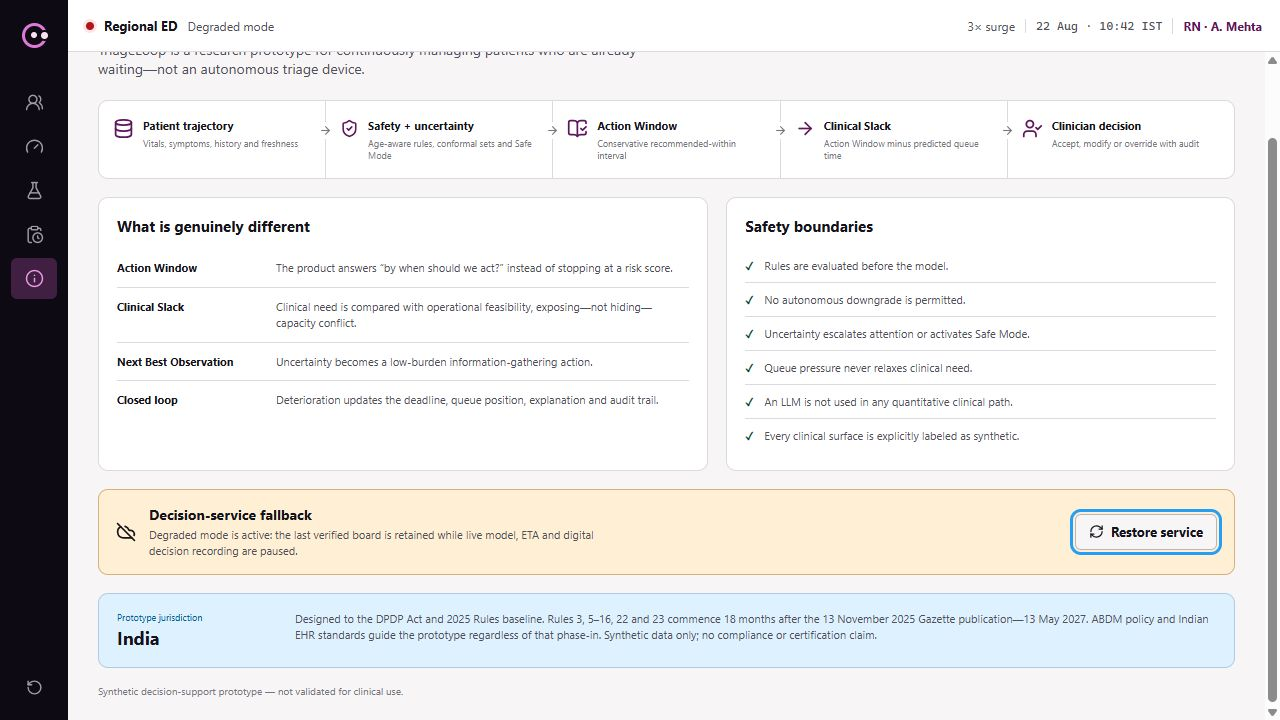
\includegraphics[width=0.82\textwidth]{../submission/visuals/product-surfaces/06-about-degraded-mode.png}
\caption{Degraded mode suppresses live estimates and actions, labels last-verified context, and directs the downtime workflow.}
\label{fig:degraded}
\end{figure}

\subsection{Audit mechanism}

Each event contains a unique ID, optional patient ID, timestamp, actor, event type, structured payload, previous hash, and event hash. With canonical serialization $c(e_k)$,

\begin{equation}
H_k=\operatorname{SHA256}\left((H_{k-1}\ \text{or GENESIS})\parallel c(e_k)\right).
\end{equation}

Integrity is reported only after recomputing every event hash and previous-link value in sequence. A direct database-tampering test verifies that modification is detected. This is tamper-evident prototype linkage, not immutable storage, non-repudiation, or a production security control.

\section{Evaluation Protocol}

\subsection{Predeclaration and research questions}

The evaluation protocol was locked before model and queue implementation to reduce metric cherry-picking. It asked whether TriageLoop could reduce missed Action Windows under crowding, preserve lower-acuity tail waits, expose uncertainty with bounded workload, use NBO to reduce observation burden without material recall loss, and remain directionally stable across age, history, site, and shift conditions.

The protocol predeclared the following prototype gates:

\begin{itemize}
  \item in-distribution critical recall at least 0.90 and stress recall at least 0.85;
  \item critical-class conformal coverage at least nominal target minus 0.03;
  \item ECE no greater than 0.08 at the selected operating horizon;
  \item at least 20\% fewer 3x-surge Action Window misses versus initial static triage;
  \item low-acuity P90 wait no more than 20\% worse than static triage unless explicitly explained;
  \item NBO at least 25\% fewer observations with no material critical-recall loss;
  \item 100\% Safe Mode activation for hard-failure fixtures and 100\% required scenario pass.
\end{itemize}

The stronger periodic comparator was added after an independent critique identified that the initial static policy did not process later observations. Its directional interpretation is reported separately; the original 20\% threshold was not silently moved to this later comparison.

\subsection{Policies}

\begin{description}[style=nextline,leftmargin=0pt]
\item[P0 - FIFO] Arrival order except immutable immediate red flags.
\item[P1 - Initial static triage] Generic five-level category and arrival order within category; no later observation processing.
\item[P1b - Fixed periodic re-triage] Every 15 minutes, accumulated observations are processed through deterministic rules/category logic; no learned trajectory risk, conformal uncertainty, Action Windows, or Slack.
\item[P2 - TriageLoop] Rules, Dynamic Action Window, uncertainty escalation, no-demotion dynamic category, Queue Twin, Slack, and bounded NBO.
\end{description}

All policies replay identical arrivals, patient trajectories, service times, and resource availability for paired comparison. Paired bootstrap intervals are computed across shift replications.

\subsection{Endpoints and reporting}

Primary endpoints are critical Action Window miss rate, unsafe under-triage, signal-to-action time, critical recall, and negative-Slack minutes. Secondary endpoints include waiting-time and rank effectiveness, wait tails by acuity, throughput, queue length, utilization, conformal coverage, calibration, abstention/review burden, alerts per waiting-patient-hour, alerts per reassessment-nurse-hour, observations requested, and subgroup gaps.

Every machine-readable result includes synthetic/simulation boundaries. Positive, neutral, and negative results are retained. The selected model artifact and evaluation files carry deterministic seeds and SHA-256 hashes.

\section{Results and Validation}

\subsection{Model and subgroup results}

The selected boosted model meets the registered synthetic horizon gates shown in Table 3. At 30 minutes, pediatric/adult/geriatric test recall is 0.963/0.969/0.991; no/partial/available-history recall is 0.975/0.978/0.971. The worst-to-best observed subgroup range is 0.028. These cohorts inherit generator assumptions and do not establish fairness or clinical generalizability.

Stress recall remains high while stress ECE rises to 0.078-0.266 across horizons. This divergence matters: high recall does not make an absolute probability calibrated under shift. The correct response is OOD/Safe Mode and future local recalibration, not a stronger confidence claim.

\subsection{Queue and operational results}

The original registered static comparison showed 36.0\% fewer 30-minute composite Action Window misses overall under 3x surge (95\% CI 31.2\%-41.1\%). Because the comparator never re-triages, this number combines the value of looking again with the value of learned dynamic prioritization. It is retained for provenance but is not the lead claim.

The lead result is the 20.5\% relative reduction against fixed 15-minute periodic re-triage. Directional benefits also appear for negative Slack, signal-to-action time, and low-acuity P90 wait. Waiting-time and rank effectiveness do not improve uniformly in every cell; the strongest evidence is deadline adherence and lateness under the declared simulation.

\subsection{NBO negative finding}

The single-observation NBO policy reduces acquisition count and assumed acquisition time substantially, but violates the fixed recall boundary. The test-selected four-observation fallback fails stress confirmation. This result is a falsified feature hypothesis, not a system failure: the evaluation did what it was designed to do and converted an appealing efficiency feature into a bounded, safer product role.

\subsection{External input plausibility}

The open MIMIC-IV Clinical Database Demo v2.2 provides a 100-patient deidentified adult hospital/ICU subset \cite{mimicdemo}. The evaluation maps 63,163 measurements across heart rate, respiratory rate, SpO2, systolic and diastolic pressure, and temperature. All five core fields are present; at least 95\% of each field lies within the prototype's hard plausibility ranges; each external median lies inside the synthetic p01-p99 interval.

This check rules out a gross unit/scale mismatch. It does not evaluate emergency-department transfer, pediatric behavior, labels, model calibration, deterioration prediction, Action Windows, queue performance, or patient outcomes. Full MIMIC-IV-ED is credentialed and was not used \cite{mimiced}.

\subsection{Engineering assurance}

The final release-candidate suite contains 73 Python tests:

\begin{table}[H]
\centering
\caption{Automated test inventory at TL-07 release candidate.}
\small
\begin{tabularx}{\textwidth}{@{}L{28mm}C{11mm}C{12mm}Y@{}}
\toprule
Test area & Files & Tests & Examples \\
\midrule
Safety & 3 & 13 & Rule precedence, Safe Mode, explanation regression, observation catalogue \\
Evaluation & 5 & 21 & TL-02 gates, queue gates, periodic comparator, NBO, external plausibility \\
Product/API & 2 & 14 & Reset, deterioration, decisions, audit integrity, security boundaries \\
Unit & 3 & 12 & Generator, features, model mechanics \\
Simulation & 1 & 6 & Queue policy, capacity and scheduling behavior \\
Contract & 1 & 4 & Strict schemas and invalid input \\
Curated scenarios & 1 & 3 & Count/coverage, ambiguity, age and zero-history cases \\
\midrule
Total & 16 & 73 & All passing \\
\bottomrule
\end{tabularx}
\end{table}

TypeScript type-check and the optimized Next.js production build pass. The isolated production rehearsal on ports 8100/3200 verified reset, deterioration, -8 minutes Slack, NBO boundary, 3x surge, reasoned override, audit integrity, evidence, and capacity without browser-console or page errors. Deliberately stopping the API produced the degraded state in Figure~\ref{fig:degraded}; explicit retry restored the live board after service restart.

Security-boundary tests reject a direct patient-name field, a 501-character override reason, unsupported DELETE reset, and malicious-origin CORS access. Frontend responses include content-type, frame, referrer, and permissions-policy headers. These are local-prototype controls; production use requires authentication, authorization, TLS, secrets management, monitored storage, and hospital-specific threat modeling.

\subsection{Reproducibility hashes}

Repeated TL-05 executions reproduced evaluation artifacts byte-for-byte. Key hashes are:

\begin{itemize}
  \item selected model: \code{b37ab29077acd37865f3a9de89c070f37bbb549f8bc13f40d819146161a51990};
  \item periodic metrics: \code{6b4bed629305c5e447c46ebfeede5725870e88b614ebb0d882f6f3ac8fdd875e};
  \item NBO metrics: \code{2c5fc3840a988c5bffce1a79f100bbf6118dd19cc65771229abc34330da7b36d};
  \item external plausibility: \code{9e92598d67fd9f2f4254b3ac468a2399e56c6cacfcd0ea90d26ab7836ce718c7}.
\end{itemize}

\section{Independent Review and Corrective Engineering}

Two external Claude reviews were conducted at deliberately different maturity points. The first five-perspective panel reviewed the scientific and architectural package before the product was complete. The second six-perspective panel reviewed the working code, evidence, rendered proposal/deck, and release package before TL-07. Neither review was treated as an instruction source. Every finding was reproduced or disproved against code, machine-readable artifacts, the running product, and authoritative sources before implementation.

\begin{figure}[H]
\centering
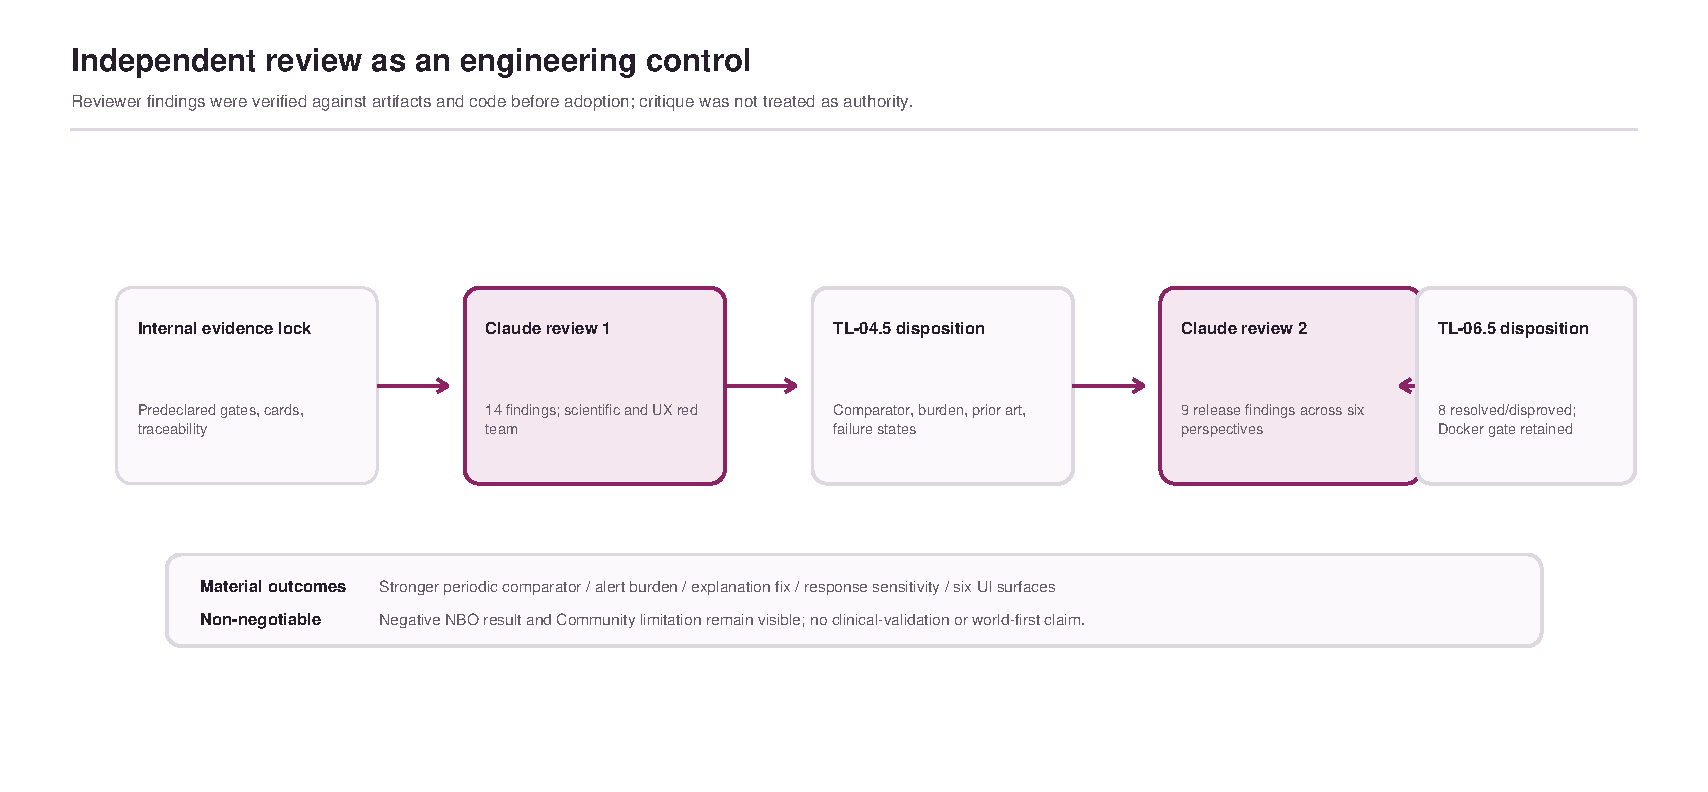
\includegraphics[width=\textwidth]{figures/review_cycle.pdf}
\caption{Independent review cycle and material corrective outcomes.}
\label{fig:reviews}
\end{figure}

\subsection{First review: pre-product red team}

The first panel scored the concept as scientifically promising but fragile. Its central criticisms were circular synthetic evidence, framing drift toward queue optimization, an unfairly weak static comparator, unresolved nurse burden, close India-focused prior art, hidden sensitivity to the response definition, undefined compound-trigger behavior, and insufficient visible product evidence.

Several ``not built'' findings became obsolete after TL-04, but the scientific findings remained valid. The corrective actions were:

\begin{itemize}
  \item reframe the story around a changing waiting patient before capacity;
  \item add the 15-minute periodic re-triage comparator;
  \item measure consolidated signals per waiting-patient-hour and reassessment-nurse-hour;
  \item cite the close India OPD prior art and narrow novelty claims;
  \item show Community separately and retain the absolute residual danger;
  \item make the synthetic evidence boundary unavoidable in the product and README;
  \item define compound-trigger precedence and degraded-mode behavior;
  \item run the NBO counterfactual rather than describing it as a benefit.
\end{itemize}

\subsection{Second review: release-candidate panel}

The final review issued a conditional go with nine findings. Eight were resolved or disproved:

\begin{longtable}{@{}L{19mm}L{37mm}L{94mm}@{}}
\caption{TL-06.5 final-review disposition.}\label{tab:review2}\\
\toprule
ID & Verdict & Verified outcome \\
\midrule
\endfirsthead
\toprule
ID & Verdict & Verified outcome \\
\midrule
\endhead
F-01 & Valid; fixed & Corrected explanation attribution; regression test requires observed oxygen/trend factors and excludes absent confusion wording. \\
F-02 & Not reproduced; strengthened & Alert evidence already existed; both denominators were surfaced consistently with Community as warning. \\
F-03 & Valid; fixed & Added periodic-comparator 10/20/30-minute sensitivity: 12.8\%/13.0\%/24.1\%. \\
F-04 & Valid; resolved at release & Docker Desktop 4.87.0, Engine 29.7.2, Compose 5.4.0 and WSL 2.7.12 were installed. The built stack passed health, full browser, restart, persistence and reset checks. \\
F-05 & Valid; fixed & Captured six working-product surfaces covering board, override, audit, evidence, capacity, and degraded mode. \\
F-06 & Not reproduced & PMID 40318497 resolves to the intended 2025 uncertainty-aware ED triage paper. \\
F-07 & Valid clarity issue; fixed & Distinguished the 1,800-shift TL-03 matrix from the 1,200-shift TL-05 matrix. \\
F-08 & Valid clarity issue; fixed & Limited ``zero findings'' to the proposal-document audit; formal product accessibility/usability remains external. \\
F-09 & Maintenance risk; fixed for release & Rechecked every source-register URL and replaced brittle links where needed. \\
\bottomrule
\end{longtable}

The review process changed implementation and claims, not just prose. It found a real explanation bug, induced a new sensitivity experiment, strengthened comparator fairness, and expanded visible product evidence. It also demonstrates an important governance pattern: independent critique is most useful when paired with a written disposition that can say \emph{accepted}, \emph{not reproduced}, \emph{superseded}, or \emph{open}, with evidence for each.

\section{Governance, Privacy, and Human Accountability}

The assumed jurisdiction is India. The governance baseline references the Digital Personal Data Protection Act 2023 and its phased Rules, the Ayushman Bharat Digital Mission Health Data Management Policy, and Indian EHR Standards \cite{dpdp,dpdprules,abdm,ehrindia}. The prototype is designed toward data minimization, purpose limitation, synthetic/pseudonymous identifiers, explicit audit events, configurable retention, and no secondary use. It does not claim legal compliance or certification.

No real patient data is required or permitted. Manual intake requires \code{provenance.synthetic=true}; unknown direct patient-name fields are rejected. The visible role label demonstrates workflow states, not production identity or authorization. A hospital deployment would require locally approved role definitions, identity federation, least privilege, encryption/key management, retention and deletion rules, consent/legal-basis analysis, incident response, monitored audit storage, and prospective clinical governance.

Human accountability is represented as state:

\begin{itemize}
  \item the recommendation remains advisory;
  \item accept, modify, and override are distinguishable actions;
  \item modify/override requires a reason;
  \item the event records recommendation ID, model/rule versions, clinician action, reason, and audit linkage;
  \item no model or queue component may autonomously downgrade, discharge, treat, or diagnose.
\end{itemize}

\section{Reproducibility and Deployment}

\subsection{Local developer workflow}

From the repository root on Python 3.12+:

\begin{lstlisting}
python -m venv .venv
.venv\Scripts\python -m pip install -e services/api
.venv\Scripts\python services/api/scripts/generate_data.py
.venv\Scripts\python services/api/scripts/train_models.py
.venv\Scripts\python services/api/scripts/run_queue_experiments.py
.venv\Scripts\python services/api/scripts/run_tl05_periodic_retriage.py
.venv\Scripts\python services/api/scripts/run_tl05_nbo.py
.venv\Scripts\python services/api/scripts/run_tl05_external_plausibility.py
Set-Location services/api
..\..\.venv\Scripts\python -m unittest discover -s ../../tests -p "test_*.py" -v
\end{lstlisting}

The API runs with Uvicorn on port 8000 and the Next.js application on port 3000. The deterministic jury path begins at \code{/board}; \emph{Run deterioration event}, \emph{3x surge}, and \emph{Reset demo} exercise the principal states.

\subsection{Container contract}

The one-command path is:

\begin{lstlisting}
docker compose up --build
\end{lstlisting}

Compose builds the Python API and standalone Next.js service. The web service starts only after the API health check at \code{/v1/health} passes. A named volume preserves prototype audit state; reset always restores the deterministic demo. The acceptance gate was to reach \code{/board} from README-only instructions on a Docker-equipped machine, exercise deterioration/override/audit, restart Compose, and verify health plus expected persistence/reset behavior.

The closing deployment pass installed Docker Desktop 4.87.0 (Engine 29.7.2, Compose 5.4.0) and WSL 2.7.12. A clean build exposed two genuine reproducibility defects before acceptance: a registry timeout could discard an incomplete pnpm install, and Next.js standalone output omitted a pnpm-linked SWC helper at runtime. The web Dockerfile was hardened with a persistent BuildKit package cache, bounded fetch retries and the resolved dependency tree in the runner image. The rebuilt stack then passed: \code{/v1/health} returned \code{ok/synthetic-prototype/0.4.0}; \code{/board} returned HTTP 200; the complete eight-state Chromium journey reported zero console and page errors; and both containers recovered after Compose restart. Five audit events and the newest SHA-256 event hash were preserved exactly across restart, chain verification remained intact, and explicit reset restored one intact baseline event. This converts the former environmental condition into a passed executable release gate rather than a static configuration claim.

\subsection{Vercel deployment architecture and live acceptance}

The UI has two explicit execution modes. In local and Docker execution, the Next.js same-origin route proxies to the live FastAPI service through \code{TRIAGELOOP\_API\_URL}; this is the reference path for scoring, recomputation, persistent audit state and manual synthetic intake. On Vercel, the same route switches to a bounded presentation adapter. The adapter serves canonical snapshots exported from the FastAPI prototype, uses an HTTP-only, same-site session cookie for small synthetic scenario flags, and appends a deterministic reasoned-decision audit event. It accepts no real patient data and does not claim to be the Python decision service.

This separation prevents two opposite errors: a jury page that renders but has no working interactions, and a hosted mock that is misrepresented as the full clinical engine. The public adapter is evidence-preserving presentation infrastructure; the Docker path remains the technical reference implementation. The environment-aware Next.js configuration retains standalone output for Docker but delegates function tracing to Vercel.

Production deployment \code{dpl\_Engkgw53P3J8XbonHm2bWbFb1vY1} reached \code{READY} and was aliased to \url{https://triageloop-ai.vercel.app}. An automated Chromium run against the public origin verified health, reset, baseline board, deterioration with negative Clinical Slack, the NBO fallback boundary, 3x surge, a reasoned override, recomputed audit-chain integrity, evaluation evidence and capacity truth. It captured eight full-page screenshots and reported zero console or page errors. The health endpoint explicitly identifies \code{synthetic-presentation-adapter}; production clinical use remains prohibited.

\section{Limitations and Threats to Validity}

\subsection{Construct validity}

The generated escalation composite combines several urgent actions. Queue conclusions depend on the response-window definition, as Figure~\ref{fig:sensitivity} demonstrates. Action Window misses are operational proxy outcomes, not patient harm. The simulator's service and arrival distributions are assumptions rather than measured local operations.

\subsection{Internal validity}

The project authors designed the generator, labels, features, model, and simulator. A model can learn the generator's own mechanisms. Patient-level isolation, untouched test data, predeclared gates, stress cohorts, and deterministic reproduction reduce leakage and selection bias but do not remove authoring circularity. The external demo checks scale only.

\subsection{External validity}

No real ED cohort was used for model performance. Pediatric external validation is absent. The MIMIC-IV demo is adult hospital/ICU data. Site profiles represent configured archetypes, not calibrated hospitals. Thresholds, rules, model calibration, subgroup behavior, workflows, and alert burden require prospective local studies.

\subsection{Human factors}

The interface has been structurally inspected and browser-tested, but no formal study with triage nurses or assistive-technology users has been completed. Alert workload is measured in simulation without an accepted safe threshold. Typical NBO acquisition time is catalogue-based, not a time-and-motion result.

\subsection{Security and regulatory readiness}

The SHA-256 chain is tamper-evident but stored locally and is not immutable. The role selector is not authentication. The prototype lacks production authorization, TLS termination, enterprise key management, retention enforcement, monitoring, backup, disaster recovery, penetration testing, and hospital integration approval. Governance references are a design baseline, not legal advice.

\subsection{Clinical-safety boundary}

The system is not a medical device, is not clinically validated, and must not be used for diagnosis, treatment, discharge, autonomous prioritization, or staffing decisions. Its rules are demonstrations requiring clinical-owner review. Negative Slack identifies an assumed capacity conflict; it does not prescribe the operational response.

\section{Prospective Validation and Product Roadmap}

The next credible step is not a larger synthetic headline. It is staged local validation:

\begin{enumerate}
  \item \textbf{Silent retrospective validation:} map local ED data, verify units/provenance, measure calibration and subgroup performance without changing care.
  \item \textbf{Shadow-mode prospective study:} run live predictions invisibly, compare Action Windows and alerts with clinician adjudication, and measure alert burden and override reasons.
  \item \textbf{Usability and safety simulation:} test time-to-comprehension, error recovery, handoff, surge, outage, and assistive technology with nurses and charge nurses.
  \item \textbf{Locally governed pilot:} expose recommendations under approved rules, monitoring, identity, audit, escalation ownership, and stop criteria.
  \item \textbf{Outcomes evaluation:} only after calibration and workflow safety are established, evaluate process and patient outcomes with an appropriate controlled design.
\end{enumerate}

Priority engineering work includes audited correction of source data, site-specific rule/configuration governance, production identity and authorization, monitored event storage, integration adapters, formal SSE/reconnect semantics, local recalibration, drift monitoring, and an NBO redesign that must pass an independent stress gate before any efficiency claim.

\section{Conclusion}

TriageLoop reframes emergency-department waiting-room triage from a one-time score into a patient-specific, capacity-aware, clinician-closed control loop. Its key design move is to translate changing clinical evidence into a conservative Action Window, keep queue feasibility separate through Clinical Slack, and make uncertainty produce a specific safe workflow rather than a decorative confidence percentage.

The synthetic evidence supports internal consistency and a positive operational hypothesis under declared assumptions. It also rejects the single-observation NBO hypothesis and reveals dependence on site capacity and response definition. Those negative and conditional results are part of the contribution. The prototype's value at this stage is not proof of clinical benefit; it is a rigorously bounded, reproducible demonstration of how safety rules, calibrated trajectory risk, uncertainty, queue feasibility, human authority, and audit can operate as one system.

\clearpage
\appendix

\section{Clinical Calculation Pseudocode}

\begin{lstlisting}
validate(patient_state, provenance, freshness, plausibility)
safety = evaluate_age_aware_rules(patient_state)

if safety.hard_red_flag:
    action = IMMEDIATE_REVIEW
    window = 0 minutes
else:
    risk = calibrated_multi_horizon_hazard(features_at_or_before_now)
    conformal_set = mondrian_prediction_set(risk)
    shifted = ood_detector(features)
    safe_mode = safety.data_quality_failure or shifted or material_ambiguity

    model_window = earliest_horizon_crossing(risk, thresholds)
    category_window = max(0, category_bound - elapsed_wait)
    window = min(model_window, category_window, safe_mode_bound)
    action = conservative_action(window, safety, clinician_state)

eta = queue_twin.projected_time_to_action(patient, current_queue, resources)
slack = window - eta
nbo = first_step_observation_only_if_decision_relevant_uncertainty

present(action, window, eta, slack, reasons, uncertainty, nbo)
clinician_decision = accept_or_modify_or_override(reason_if_required)
append_and_recompute_hash_linked_audit(clinician_decision)
\end{lstlisting}

\section{API Surface}

\begin{longtable}{@{}L{43mm}L{24mm}L{82mm}@{}}
\toprule
Endpoint & Method & Purpose \\
\midrule
\endfirsthead
\toprule
Endpoint & Method & Purpose \\
\midrule
\endhead
\code{/v1/health} & GET & Health, prototype mode, and API version \\
\code{/v1/config} & GET & Site/scenario configuration and safety boundaries \\
\code{/v1/demo/state} & GET & Complete deterministic board state \\
\code{/v1/demo/reset} & POST & Restore baseline fixtures and audit genesis \\
\code{/v1/demo/scenario} & POST & Select baseline or 3x surge \\
\code{/v1/demo/deteriorate/\{id\}} & POST & Apply registered repeated-observation hero event \\
\code{/v1/intake/manual} & POST & Strict synthetic manual intake \\
\code{/v1/patients/\{id\}/recommendation} & GET & Recommendation envelope with risk, uncertainty, Window, Slack, NBO, explanation \\
\code{/v1/patients/\{id\}/decisions} & POST & Accept, modify, or override; reason required where applicable \\
\code{/v1/audit} & GET & Ordered material event history \\
\code{/v1/audit/integrity} & GET & Full recomputation of hash and previous-link integrity \\
\code{/v1/evaluations/latest} & GET & Machine-readable model, queue, NBO, and plausibility evidence \\
\code{/v1/events/stream} & GET & Server-sent state/heartbeat stream \\
\bottomrule
\end{longtable}

\section{Claim-Control Ledger}

\begin{longtable}{@{}L{48mm}L{43mm}L{58mm}@{}}
\toprule
Permitted claim & Required qualifier & Prohibited expansion \\
\midrule
\endfirsthead
\toprule
Permitted claim & Required qualifier & Prohibited expansion \\
\midrule
\endhead
20.5\% fewer Action Window misses & Synthetic 3x-surge simulation versus fixed 15-minute periodic re-triage; 95\% CI 17.4\%-23.8\% & Patient benefit, mortality reduction, or real-hospital performance \\
NBO requested 87.5\% fewer observations & It lost 7.1 recall points and failed; first-step only & Workload reduction with preserved safety \\
63,163 external measurements mapped & Open adult hospital/ICU demo; input scale only & External model validation or ED transfer \\
Critical recall/coverage gates pass & Generated test/stress cohorts & Clinical accuracy, fairness, or regulatory performance \\
Hash chain detects tampering & Local prototype recomputation & Immutable, certified, or non-repudiable audit \\
Structural accessibility checks pass & Browser/DOM and stylesheet inspection & Formal WCAG conformance or nurse usability \\
India governance baseline used & Design framing only & DPDP/ABDM legal compliance or certification \\
\bottomrule
\end{longtable}

\section{Artifact and Evidence Map}

\begin{longtable}{@{}L{54mm}L{104mm}@{}}
\toprule
Artifact & Role in this monograph \\
\midrule
\endfirsthead
\toprule
Artifact & Role in this monograph \\
\midrule
\endhead
\code{docs/clinical-safety-contract.md} & Safety invariants, authority, failure and audit boundaries \\
\code{docs/evaluation-protocol.md} & Predeclared research questions, endpoints, gates, model-selection rule \\
\code{docs/model-card.md} & Data isolation, selected-model results, uncertainty and limitations \\
\code{docs/simulation-card.md} & Site/load assumptions, policy definitions, queue evidence and limits \\
\code{docs/requirements-traceability.md} & Official-brief requirement-to-evidence mapping \\
\code{docs/tl-04.5-critique-disposition.md} & First independent-review verification and corrective actions \\
\code{docs/tl-06.5-final-review-disposition.md} & Final panel finding-by-finding resolution \\
\code{docs/tl-05-verification-report.md} & Scientific, product, security, accessibility, and reproducibility checkpoint \\
\code{docs/tl-07-release-report.md} & Final local full-story, test/build, video, and release-package evidence \\
\code{artifacts/release/tl07-docker-verification.json} & Docker versions, endpoint/browser results, restart persistence, reset contract, and fixes found by the gate \\
\code{paper/diagrams/*.mmd} & Editable Mermaid sources for the system architecture, runtime clinical-decision flow, and ML-development pipeline blueprints \\
\code{artifacts/evaluation/tl-02-metrics.json} & Candidate/selected model metrics and subgroup evidence \\
\code{artifacts/evaluation/tl-03-queue-metrics.json} & Original 1,800-shift matrix and static comparator \\
\code{artifacts/evaluation/tl-05-periodic-retriage-metrics.json} & Stronger 1,200-shift comparator, sensitivity, and workload \\
\code{artifacts/evaluation/tl-05-nbo-metrics.json} & Failed NBO gate and fallback sensitivity \\
\code{artifacts/evaluation/tl-05-external-plausibility.json} & Open-reference input-scale checks \\
\code{submission/visuals/product-surfaces/} & Six direct working-product evidence captures \\
\bottomrule
\end{longtable}

\section{Reproduction Checklist}

\begin{enumerate}
  \item Confirm Python 3.12+, Node 22+, pnpm, and optional Docker Desktop.
  \item Rebuild generated encounters with seed \code{20260821}; confirm snapshot counts and manifest.
  \item Retrain candidates; confirm selected model family and model SHA-256.
  \item Rerun original queue, periodic comparator, NBO, and external-plausibility scripts.
  \item Compare evaluation hashes with the recorded values.
  \item Run all 73 Python tests, TypeScript check, and optimized Next.js build.
  \item Start API/web; execute reset, deterioration, surge, override, audit, evidence, capacity, and outage/recovery.
  \item With Docker, follow the README Compose steps; verify health, board, restart/persistence, and reset.
  \item For Vercel, connect the API and restrict CORS. Verify the synthetic workflow from the public deployment.
  \item Recheck all external links and retain the synthetic/non-clinical boundary on every public artifact.
\end{enumerate}

\clearpage
\small
\begin{thebibliography}{99}

\bibitem{accenturebrief}
Accenture Innovation Challenge 2026. \emph{Round 2 - Prototype Development: PatientTriage.ai}. Supplied competition brief, pp. 2-4, 2026.

\bibitem{quinten2018}
V. M. Quinten, M. van Meurs, T. J. Olgers, J. M. Vonk, J. J. M. Ligtenberg, and J. C. ter Maaten. ``Repeated vital sign measurements in the emergency department predict patient deterioration within 72 hours: a prospective observational study.'' \emph{Scandinavian Journal of Trauma, Resuscitation and Emergency Medicine}, 26:57, 2018. doi:10.1186/s13049-018-0525-y.

\bibitem{brekke2019}
I. J. Brekke et al. ``The value of vital sign trends in predicting and monitoring clinical deterioration: A systematic review.'' \emph{PLOS ONE}, 14(1), 2019. PMID 30645637.

\bibitem{timevarying2026}
``A High-Precision Time-Varying Survival Model for Early Prediction of Patient Deterioration: A Retrospective Cohort Study.'' PubMed PMID 41827109, 2026. \url{https://pubmed.ncbi.nlm.nih.gov/41827109/}.

\bibitem{traumaranking2023}
``Development of an Anticipatory Triage-Ranking Algorithm Using Dynamic Simulation of the Expected Time Course of Patients With Trauma: Modeling and Simulation Study.'' PubMed PMID 37318826, 2023. \url{https://pubmed.ncbi.nlm.nih.gov/37318826/}.

\bibitem{angelopoulos2023}
A. N. Angelopoulos and S. Bates. ``Conformal Prediction: A Gentle Introduction.'' \emph{Foundations and Trends in Machine Learning}, 16(4):494-591, 2023. doi:10.1561/2200000101.

\bibitem{abdulai2025}
A. S. B. Abdulai, J. Storm, and M. Ehrlich. ``I don't know: An uncertainty-aware machine learning model for predicting patient disposition at emergency department triage.'' \emph{International Journal of Medical Informatics}, 201:105957, 2025. doi:10.1016/j.ijmedinf.2025.105957.

\bibitem{nasaRUL}
NASA. \emph{Prognostics and Remaining Useful Life research reference}. NASA Technical Reports Server, 2014. \url{https://ntrs.nasa.gov/api/citations/20140010623/downloads/20140010623.pdf}.

\bibitem{liu1973}
C. L. Liu and J. W. Layland. ``Scheduling Algorithms for Multiprogramming in a Hard-Real-Time Environment.'' \emph{Journal of the ACM}, 20(1):46-61, 1973.

\bibitem{ibmafa}
IBM Research. \emph{Active Feature Acquisition}. Research project overview. \url{https://research.ibm.com/projects/active-feature-acquisition}. Accessed 22 August 2026.

\bibitem{whotriage}
World Health Organization. \emph{Interagency Integrated Triage Tool}. \url{https://www.who.int/tools/triage}. Accessed 22 August 2026.

\bibitem{gupta2026}
R. Gupta, A. Kumar, and S. Dang. ``Agentic AI for Clinical Urgency Mapping and Queue Optimization in High-Volume Outpatient Departments: A Simulation-Based Evaluation.'' arXiv:2604.00215, 2026. \url{https://arxiv.org/abs/2604.00215}.

\bibitem{mimicdemo}
PhysioNet. \emph{MIMIC-IV Clinical Database Demo, version 2.2}. DOI 10.13026/dp1f-ex47. \url{https://physionet.org/content/mimic-iv-demo/2.2/}.

\bibitem{mimiced}
PhysioNet. \emph{MIMIC-IV-ED, version 2.2}. Credentialed data resource. \url{https://physionet.org/content/mimic-iv-ed/2.2/}.

\bibitem{dpdp}
Government of India. \emph{Digital Personal Data Protection Act, 2023}. India Code. \url{https://www.indiacode.nic.in/handle/123456789/22037}.

\bibitem{dpdprules}
Ministry of Electronics and Information Technology. \emph{Digital Personal Data Protection Rules, 2025}. Government of India. \url{https://www.meity.gov.in/}.

\bibitem{abdm}
National Health Authority. \emph{Ayushman Bharat Digital Mission Health Data Management Policy}. \url{https://abdm.gov.in/}.

\bibitem{ehrindia}
Ministry of Health and Family Welfare. \emph{Electronic Health Record Standards for India}. Government of India, 2016. \url{https://www.mohfw.gov.in/}.

\end{thebibliography}

\normalsize
\vspace{5mm}
\begin{center}
\colorbox{TBrandSoft}{\parbox{0.92\textwidth}{\centering\vspace{2mm}\textbf{Final boundary:} TriageLoop is a synthetic research and product prototype. It does not autonomously diagnose, treat, discharge, downgrade, determine staffing, or replace licensed clinical judgment.\vspace{2mm}}}
\end{center}

\end{document}
